%Version 3.1 December 2024 -- plantilla Springer Nature (sn-jnl)
%
% Proyecto 2026-30 -- Analisis de Algoritmos -- Pontificia Universidad Javeriana
% Entrega 1: Diseno y estrategia de datos
%
% Archivos que acompanan este .tex (subirlos a Overleaf junto a sn-jnl.cls):
%   carpeta figuras/  (diagramas en PDF y mockups en PNG)
%   sn-bibliography.bib  (reemplaza al de la plantilla)

\documentclass[pdflatex,sn-mathphys-num]{sn-jnl}% Math and Physical Sciences Numbered Reference Style

%%%% Paquetes estandar de la plantilla
\usepackage{graphicx}%
\usepackage{multirow}%
\usepackage{amsmath,amssymb,amsfonts}%
\usepackage{amsthm}%
\usepackage{mathrsfs}%
\usepackage[title]{appendix}%
\usepackage{xcolor}%
\usepackage{textcomp}%
\usepackage{manyfoot}%
\usepackage{booktabs}%
\usepackage{listings}%
%%%% Paquetes adicionales
\usepackage[utf8]{inputenc}%
\usepackage[T1]{fontenc}%
\usepackage[spanish,es-noshorthands,es-nodecimaldot,es-tabla]{babel}%
\usepackage{tabularx}%
\usepackage{array}%
\usepackage{float}
\usepackage{placeins}
\renewcommand{\keywordname}{Palabras clave}
\hypersetup{hypertexnames=false}
%% Columnas de tabla con texto alineado a la izquierda
\newcolumntype{L}{>{\raggedright\arraybackslash}X}

%% Estilo de los ejemplos JSON
\lstdefinestyle{json}{
  basicstyle=\ttfamily\scriptsize,
  columns=fullflexible,
  breaklines=true,
  frame=single,
  framesep=4pt,
  showstringspaces=false,
  literate={á}{{\'a}}1 {é}{{\'e}}1 {í}{{\'i}}1 {ó}{{\'o}}1 {ú}{{\'u}}1 {ñ}{{\~n}}1
}

\raggedbottom

\begin{document}

\title[Asignación de horarios estudiantiles]{Asignación de horarios estudiantiles con preferencias: diseño y estrategia de datos}

\author[1]{\fnm{Andrés José} \sur{Castrillo Torres}}
\email{ancastrillo@javeriana.edu.co}

\author[1]{\fnm{Sebastián} \sur{Vargas Casquete}}
\email{se.vargas@javeriana.edu.co}

\affil[1]{%
    \orgdiv{Ingeniería de Sistemas},
    \orgname{Pontificia Universidad Javeriana},
    \orgaddress{\city{Bogotá}, \country{Colombia}}%
}

\abstract{Este documento presenta el diseño de un sistema que asigna secciones de materias a un grupo de estudiantes. El sistema tiene en cuenta cupos, créditos, cruces de horario, disponibilidad y tiempos de traslado. Primero busca atender las materias de prioridad 5, luego las de prioridad 4 y así hasta 1. Si hay empate, puede dar prioridad por semestre; después considera las preferencias sobre horarios, profesores y compañeros. Se define qué datos recibe, qué resultados debe entregar y qué reglas deben cumplirse. También se propone cómo crear datos de prueba, obtener respuestas esperadas y comprobar la calidad de las asignaciones. Se propone un desarrollo por diez niveles y se describe la aplicación web para cargar datos y consultar horarios. Esta primera entrega corresponde al diseño y al plan de pruebas; la implementación se realizará en la siguiente etapa.}

\keywords{asignación de horarios, restricciones, optimización lexicográfica, datos sintéticos, verificación de algoritmos}

\maketitle

%%==================================================================%%
\section{Introducción}\label{sec:intro}

Organizar un horario requiere encontrar secciones que permitan cursar las materias necesarias sin cruces y con cupos disponibles. La decisión también afecta a otros estudiantes: una persona puede ocupar el único cupo que le sirve a otra, aunque tenga varias alternativas. A esto se suman preferencias sobre profesores, tiempos libres, cercanía de salones y compañeros.

El proyecto de Análisis de Algoritmos 2026-30 pide diseñar un algoritmo para asignar horarios a un conjunto de estudiantes. Para la primera entrega solicita dos cosas: definir con precisión las entradas y salidas, sin depender del algoritmo elegido, y proponer cómo obtener los datos de prueba y sus respuestas esperadas \cite{enunciado}.

La propuesta parte de una oferta de secciones con profesores, horarios y salones ya definidos. Cada estudiante indica qué materias necesita y les asigna una prioridad de 1 a 5. Se comparan primero las materias atendidas de prioridad 5; solo si hay empate se pasa a la prioridad 4, y así hasta 1. Después puede usarse el semestre como desempate y, finalmente, las preferencias personales.

Las Secciones~\ref{sec:formal} y~\ref{sec:datos} desarrollan los dos puntos principales de esta entrega. Las demás describen el sistema, los datos, la propuesta de desarrollo y la interfaz. Los límites de horas y créditos son supuestos del equipo para este proyecto. La implementación y las pruebas del programa corresponden a la segunda entrega.

%%==================================================================%%
\section{Descripción del sistema}\label{sec:sistema}

\subsection{Qué hace}

El sistema recibe la \textbf{oferta} del semestre (materias, secciones, profesores y edificios) y las \textbf{solicitudes y preferencias} de los estudiantes, y en una sola corrida decide qué sección de cada materia le corresponde a cada uno. La salida final debe cumplir las reglas obligatorias y, dentro de ellas, el sistema busca primero inscribir la mayor cantidad posible de materias importantes y después respetar las preferencias personales.

En este documento, una \emph{materia} es lo que el estudiante quiere cursar (por ejemplo, Cálculo~I) y una \emph{sección} es una oferta concreta de esa materia, con profesor, horario y cupo (por ejemplo, Cálculo~I grupo~02); en el día a día a la sección también se le llama ``clase''.

La asignación se hace \textbf{por lotes}, considerando a todos los estudiantes a la vez, y no por orden de llegada. Esto permite mover estudiantes entre secciones para dejar cupos a quienes tienen menos alternativas. La propuesta intentará mejorar el reparto, aunque no asegura encontrar siempre el mejor.

\subsection{Usuarios}

\begin{itemize}
\item \textbf{Estudiante.} Usuario principal. Declara sus materias, sus horas ocupadas y sus preferencias, y consulta el horario que le quedó.
\item \textbf{Universidad.} Carga la oferta, ajusta los parámetros generales y lanza las corridas.
\item \textbf{Profesor.} No usa el sistema; aparece como dato de cada sección y como objeto de las preferencias de los estudiantes.
\end{itemize}

\subsection{Supuestos y decisiones de diseño}\label{sec:supuestos}

\begin{itemize}
\item Las clases son de lunes a sábado, entre las \textbf{07:00 y las 20:00}. Cada sesión de clase dura \textbf{2 horas} y empieza en hora en punto, de modo que la última sesión del día empieza a las 18:00.
\item Una clase termina \textbf{10 minutos} antes de su hora oficial; ese es el tiempo para cambiar de salón.
\item Los créditos pertenecen a la materia: todas sus secciones valen lo mismo. Cada materia vale entre 1 y 6 créditos y \textbf{todo estudiante puede inscribir como máximo 20 créditos}.
\item La información se guarda en \textbf{archivos JSON locales}, no en una base de datos; se actualiza editando esos archivos o desde la aplicación.
\item La aplicación \textbf{no tiene inicio de sesión}: se elige el estudiante en un selector, lo que evita entrar y salir por cada uno.
\item No se validan prerrequisitos, no se asignan salones ni profesores (vienen en la oferta) y no hay inscripción en tiempo real ni listas de espera.
\end{itemize}

%%==================================================================%%
\section{Requerimientos}\label{sec:req}

Los requerimientos se dividen en \emph{reglas obligatorias}, que nunca se violan, y \emph{preferencias}, que se intentan cumplir pero pueden ceder. La última columna indica en qué nivel del algoritmo (Sección~\ref{sec:niveles}) se incorpora cada una.

\begin{table}[hbtp]
\caption{Reglas obligatorias}\label{tab:reglas}
\small
\begin{tabularx}{\textwidth}{@{}llLc@{}}
\toprule
ID & Regla & Descripción & Nivel \\
\midrule
R1 & Solo lo solicitado & Se inscriben solo las materias pedidas o sus sustitutas & N1 \\
R2 & Una sección por materia & Nadie queda en dos secciones de la misma materia & N1 \\
R3 & Sin choques & Las clases de un estudiante no se cruzan & N1 \\
R4 & Cupos & Ninguna sección supera su cupo & N1 \\
R5 & Tope de créditos & Nadie supera 20 créditos & N2 \\
R6 & Franjas obligatorias & Ninguna clase cae en una franja que el estudiante marcó como no disponible (por ejemplo, trabajo) & N2 \\
R7 & Profesores vetados & Nunca se asigna una sección de un profesor vetado & N2 \\
R8 & Traslado posible & Entre dos clases seguidas hay tiempo para caminar de un edificio al otro & N3 \\
R9 & Sustituta excluyente & Una sustituta solo se inscribe si la materia principal no quedó & N4 \\
\botrule
\end{tabularx}
\end{table}

\begin{table}[htbp]
\caption{Preferencias}\label{tab:prefs}
\small
\begin{tabularx}{\textwidth}{@{}llLc@{}}
\toprule
ID & Preferencia & Descripción & Nivel \\
\midrule
P1 & Prioridad de materias & De 1 (``puedo vivir sin ella'') a 5 (``la necesito''); decide qué se atiende primero & N1 \\
P2 & Materias sustitutas & Otra materia que se acepta si la principal no cabe & N4 \\
P3 & Afinidad con profesores & De $-2$ a $+2$ por profesor; el veto (R7) se declara por separado & N5 \\
P4 & Horario ideal & Franjas preferidas (por ejemplo, mañanas) y franjas a evitar & N6 \\
P5 & Franjas libres deseables & Por ejemplo, de 13:00 a 14:00 para almorzar & N6 \\
P6 & Evitar huecos & Pocas horas muertas entre clases (peso bajo) & N6 \\
P7 & Salones cerca & Poca caminata entre clases seguidas & N7 \\
P8 & Importancia personal & Alta, media o baja para cada criterio & N8 \\
P9 & Amigos y personas a evitar & Quedar o no en la misma sección que otros estudiantes & N9 \\
P10 & Prioridad institucional & Desempate por semestre si se activa, después de comparar las materias atendidas & N10 \\
\botrule
\end{tabularx}
\end{table}

\subsection{Cómo se decide qué asignación es mejor}\label{sec:mejor}

Primero se comprueba que el horario cumpla todas las reglas obligatorias. Después se comparan las materias atendidas, empezando por las de prioridad 5 y siguiendo hasta 1. Una principal inscrita cuenta 1 y una sustituta cuenta 0,8 dentro de la prioridad de su solicitud.

Si los resultados empatan en las cinco prioridades, puede usarse el semestre para decidir, si esa opción está activada. Las preferencias personales se comparan después. Por ejemplo, tener las clases en la mañana no justifica perder una materia más prioritaria. La Sección~\ref{sec:objetivo} explica el cálculo y la Sección~\ref{sec:metricas} indica cómo medir las preferencias.

\subsection{Qué pasa cuando no se puede cumplir}\label{sec:fallos}

Si una materia no cabe tal como se pidió, el sistema prueba otras secciones y luego las sustitutas. Si tampoco puede asignarla, genera un \textbf{aviso} con la causa y una sugerencia (Tabla~\ref{tab:causas}). Cuando hay varias causas, registra todas y destaca la más frecuente; si empatan, usa el número de regla.

El aviso explica lo ocurrido en el horario obtenido. No asegura que sea imposible encontrar otra asignación mejor. Si el algoritmo dejó pasar una alternativa válida, se indica como limitación del algoritmo. Solo se dice que un cupo se cedió por semestre cuando la decisión quedó registrada.

\begin{table}[htbp]
\caption{Causas de no inscripción}\label{tab:causas}
\small
\begin{tabularx}{\textwidth}{@{}lLL@{}}
\toprule
Causa & Significado & Sugerencia \\
\midrule
Sin secciones & La materia no tiene secciones en la oferta & Revisar el código de la materia \\
Cupo lleno & Todas las secciones compatibles están llenas & Revisar alternativas y oferta de cupos \\
Choque de horario & Las alternativas chocan con el horario obtenido & Revisar secciones y prioridades declaradas \\
Tope de créditos & Inscribirla superaría los 20 créditos & Quitar una materia de menor prioridad \\
Franja obligatoria & Todas las secciones caen en horas no disponibles & Revisar las franjas obligatorias \\
Profesor vetado & Todas las secciones son de profesores vetados & Cambiar el veto por una afinidad negativa \\
Traslado imposible & No hay tiempo para caminar entre edificios & Aceptar otra franja \\
Cedida por prioridad & El cupo se dio a un estudiante con prioridad institucional mayor & --- \\
\botrule
\end{tabularx}
\end{table}

%%==================================================================%%
\section{Tipos abstractos de datos}\label{sec:tads}

Primero se define cada TAD por separado, con sus atributos, invariantes y operaciones (Figuras~\ref{fig:tads-oferta} y~\ref{fig:tads-estudiante}), y después se muestra cómo se relacionan (Figura~\ref{fig:relaciones}). Las horas se escriben en formato de 24 horas y los días son L, M, X, J, V y S.

\begin{figure}[htbp]
\centering
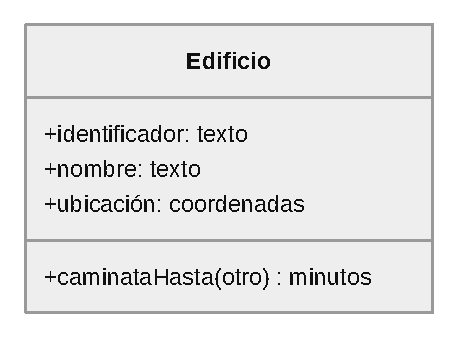
\includegraphics[width=0.35\textwidth]{figuras/tad_edificio.pdf}\hfill
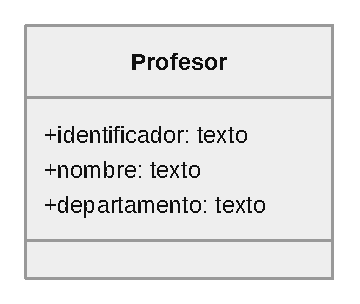
\includegraphics[width=0.31\textwidth]{figuras/tad_profesor.pdf}\hfill
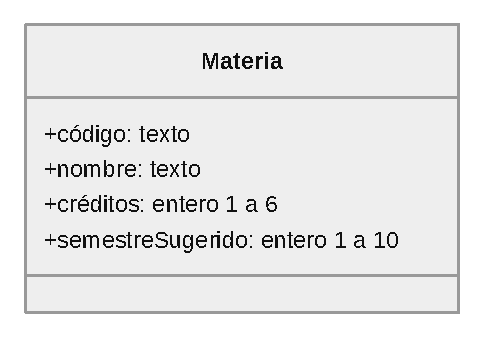
\includegraphics[width=0.34\textwidth]{figuras/tad_materia.pdf}

\vspace{10pt} % Espacio vertical entre las dos filas

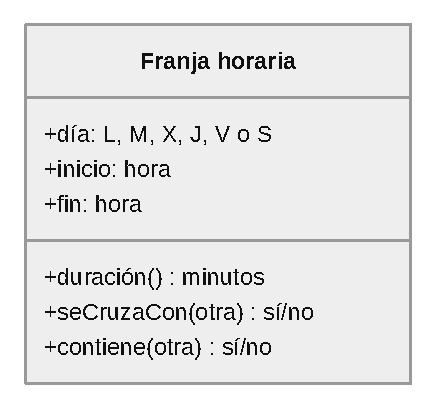
\includegraphics[width=0.31\textwidth]{figuras/tad_franja.pdf}\hfill
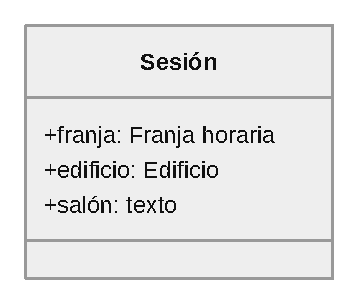
\includegraphics[width=0.31\textwidth]{figuras/tad_sesion.pdf}\hfill
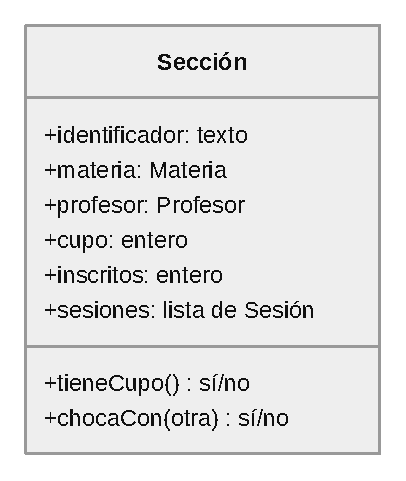
\includegraphics[width=0.31\textwidth]{figuras/tad_seccion.pdf}
\caption{TADs de la oferta: Edificio, Profesor, Materia, Franja horaria, Sesión y Sección.}\label{fig:tads-oferta}
\end{figure}

\paragraph{Edificio.} Un lugar del campus, con identificador único, nombre y ubicación aproximada. Su operación \emph{caminataHasta(otro)} devuelve los minutos para llegar a otro edificio; desde el mismo edificio es 0 y el tiempo es igual en ambos sentidos.

\paragraph{Profesor.} Identificador único, nombre y departamento. Invariante: un profesor nunca tiene dos secciones a la misma hora.

\paragraph{Materia.} Código único, nombre, créditos (de 1 a 6) y semestre sugerido (de 1 a 10).

\paragraph{Franja horaria.} Un día con una hora de inicio y una de fin. Invariante: el inicio es anterior al fin y ambos son horas en punto entre las 07:00 y las 20:00. Operaciones: \emph{duración()}; \emph{seCruzaCon(otra)}, verdadera si son el mismo día y los intervalos se solapan; y \emph{contiene(otra)}, verdadera si la otra cabe completa dentro de esta.

\paragraph{Sesión.} Un bloque semanal de clase: una franja horaria, un edificio y un salón. Invariante: su franja dura exactamente 2 horas.

\paragraph{Sección.} Una oferta concreta de una materia: identificador, materia, profesor, cupo, número de inscritos y una o más sesiones. Invariantes: el cupo es mayor que cero, los inscritos nunca superan el cupo y las sesiones de la sección no se cruzan entre sí. Operaciones: \emph{tieneCupo()}, verdadera si inscritos $<$ cupo; y \emph{chocaCon(otra)}, verdadera si alguna sesión se cruza con alguna de la otra sección.

\begin{figure}[htbp]
\centering
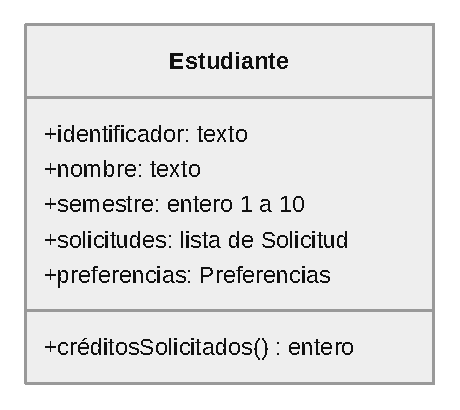
\includegraphics[width=0.48\textwidth]{figuras/tad_estudiante.pdf}\hfill
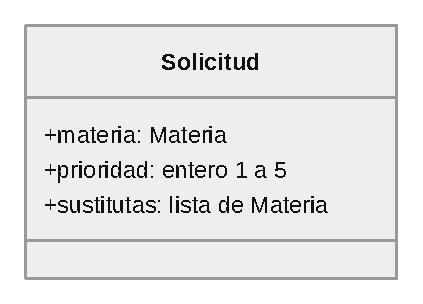
\includegraphics[width=0.48\textwidth]{figuras/tad_solicitud.pdf}

\vspace{10pt} % Espaciado vertical entre filas

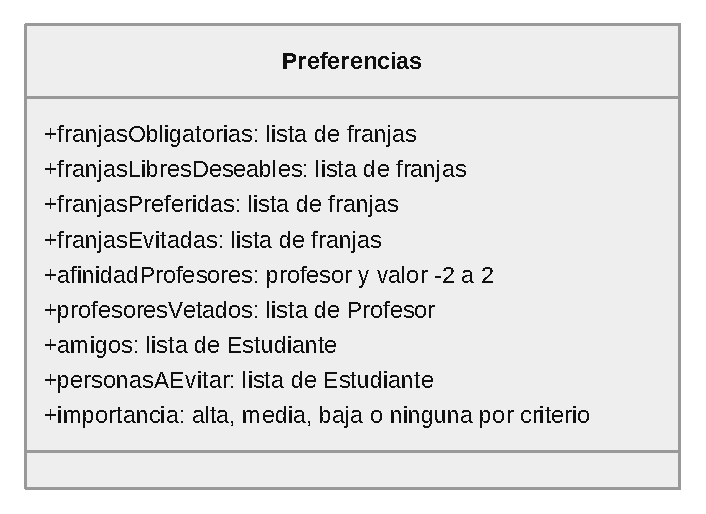
\includegraphics[width=0.48\textwidth]{figuras/tad_preferencias.pdf}\hfill
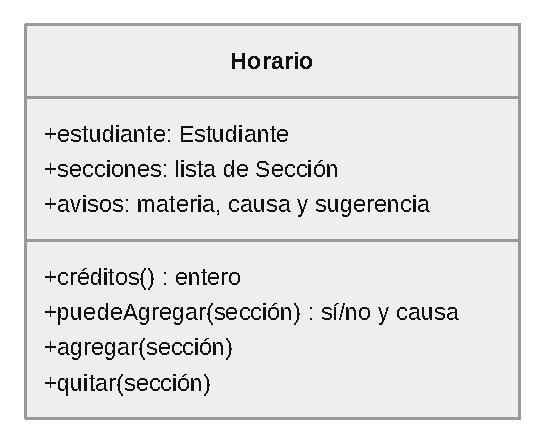
\includegraphics[width=0.48\textwidth]{figuras/tad_horario.pdf}
\caption{TADs del estudiante: Estudiante, Solicitud, Preferencias y Horario.}\label{fig:tads-estudiante}
\end{figure}

\paragraph{Estudiante.} Identificador único, nombre, semestre (de 1 a 10), sus solicitudes y sus preferencias. Invariantes: no pide dos veces la misma materia y no tiene preferencias sociales hacia sí mismo. Operación: \emph{créditosSolicitados()}.

\paragraph{Solicitud.} Una materia pedida, su prioridad (de 1 a 5) y una lista ordenada de sustitutas, que puede estar vacía. Invariante: una sustituta no puede ser también una materia pedida por el mismo estudiante.

\paragraph{Preferencias.} Las franjas obligatoriamente libres y las libres deseables; las franjas preferidas y las que quiere evitar; la afinidad con profesores (de $-2$ a $+2$) y los vetados; los amigos y las personas a evitar; y la importancia (alta, media, baja o ninguna) de cada criterio. Todas son opcionales; los criterios sin información se excluyen del promedio de preferencias, según la Sección~\ref{sec:metricas}. La afinidad negativa no equivale a veto.

\paragraph{Horario.} El resultado para un estudiante: sus secciones inscritas y los avisos de las materias que no pudo inscribir. Invariante: siempre cumple las reglas obligatorias activas. Operaciones: \emph{créditos()}; \emph{puedeAgregar(sección)}, que dice si la sección cabe o, si no, la causa; \emph{agregar(sección)}, cuya precondición es que pueda agregarse y cuya postcondición es que la sección queda en el horario y sus inscritos aumentan en uno; y \emph{quitar(sección)}, que deshace lo anterior.

\subsection{Relaciones entre los TADs}

\begin{figure}[H]
\centering
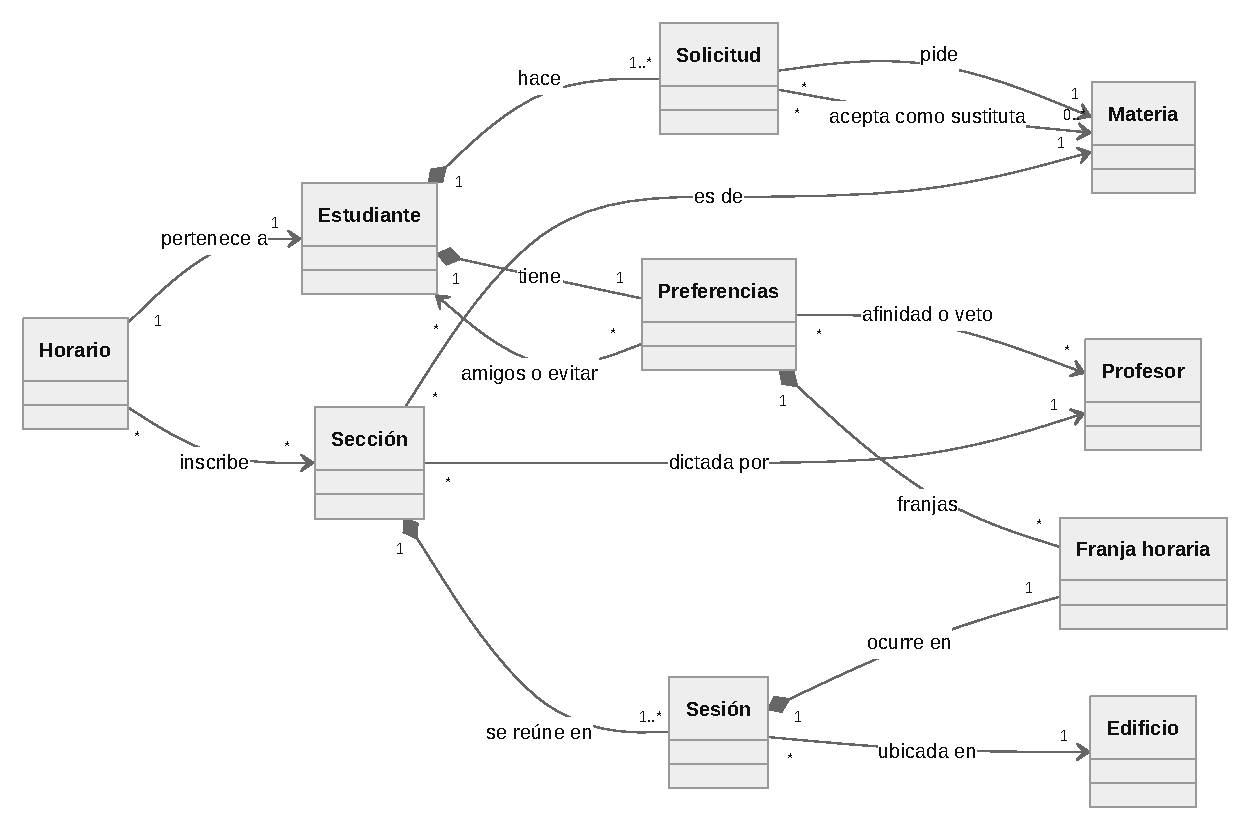
\includegraphics[width=\textwidth]{figuras/relaciones.pdf}
\caption{Relaciones entre los TADs.}\label{fig:relaciones}
\end{figure}

La Figura~\ref{fig:relaciones} resume cómo se conectan. Una \emph{sección} es de una materia, la dicta un profesor y se reúne en una o más \emph{sesiones}, cada una con su franja horaria y su edificio. Un \emph{estudiante} hace cero o más \emph{solicitudes}, cada una de una materia y con sus posibles sustitutas, y tiene unas \emph{preferencias} que apuntan a franjas, profesores y otros estudiantes. El \emph{horario} de cada estudiante es lo que produce el algoritmo: une al estudiante con las secciones que le fueron asignadas. Los diagramas resumen el diseño. También se admite un estudiante sin solicitudes y, al modificar un horario, se registra qué solicitud atiende cada sección.

%%==================================================================%%
\section{Definición del problema}\label{sec:formal}

\subsection{Entradas}

Una \emph{instancia} es el conjunto de datos de una ejecución. Recibe la oferta (materias, profesores y secciones), los edificios y tiempos de traslado, los estudiantes con sus solicitudes y preferencias, y la configuración. Sus atributos y rangos son los definidos en los TADs de la Sección~\ref{sec:tads}: créditos de 1 a 6, semestres de 1 a 10, prioridades de 1 a 5, afinidades de $-2$ a $+2$ y cupos enteros positivos.

Las sesiones son de lunes a sábado, entre 07:00 y 20:00, duran dos horas y empiezan en hora en punto. Para cada par de edificios se indican minutos enteros de caminata, mayores o iguales a cero; ir y volver toma lo mismo y dentro del mismo edificio el tiempo es cero.

Cada estudiante puede tener cero o más solicitudes. No repite principales y sus listas de sustitutas no contienen materias repetidas ni ninguna de sus principales. Una sustituta puede aparecer en varias listas, pero inscribirla solo atiende una solicitud. Las preferencias son opcionales; el día \texttt{*} se interpreta como lunes a sábado.

La configuración fija 20 créditos como máximo, valor de sustitución de 0,8 y activación o desactivación del desempate por semestre. Para repetir una prueba se guardan además semilla, nivel y versión del programa. Cada ejecución empieza con cero inscritos y reparte los cupos entre los estudiantes incluidos.

\subsection{Salidas}

Sea $S$ el conjunto de secciones y $R_e$ el de solicitudes del estudiante $e$. El resultado asigna a cada solicitud una sección o ninguna:
\[
a_e:R_e\longrightarrow S\cup\{\varnothing\}.
\]
$a_e(r)=s$ significa que la sección $s$ atiende la solicitud $r$; $\varnothing$ indica que quedó pendiente. El horario reúne las secciones asignadas al estudiante.

Cada solicitud tiene un estado: \emph{principal inscrita}, \emph{sustituida} o \emph{no inscrita}. Los dos últimos generan exactamente un aviso con causa y sugerencia. La salida conserva qué solicitud atendió cada sección e incluye créditos, inscritos por sección, atención por prioridad y satisfacción de preferencias. El resumen informa solicitudes atendidas y pendientes, reglas incumplidas y tiempo de ejecución. Se guardan las entradas y la configuración usadas.

\subsection{Restricciones}

Todo resultado debe cumplir R1--R9 de la Tabla~\ref{tab:reglas}, para cada estudiante y sección:
\begin{enumerate}
\item Asignar solo principales o sustitutas aceptadas, con una sección como máximo por solicitud y una inscripción como máximo por materia.
\item No superar el cupo de ninguna sección ni los 20 créditos por estudiante. Una sustituta cuenta con sus propios créditos.
\item Evitar cruces, franjas obligatoriamente libres y profesores vetados. Dos sesiones se cruzan si son el mismo día y cada una empieza antes de que termine la otra. Así, 07:00--09:00 y 09:00--11:00 no se cruzan. Una afinidad negativa no equivale a veto.
\item Permitir el traslado entre sesiones consecutivas: el tiempo de caminata no puede superar los minutos libres entre ellas más diez minutos de salida anticipada. Con clases seguidas hay diez minutos; con una hora libre, setenta. Esto no autoriza cruces en los horarios oficiales.
\end{enumerate}

La primera condición impide asignar una principal y su sustituta simultáneamente o contar una inscripción para dos solicitudes. Estas reglas describen un resultado válido independientemente del algoritmo que lo construya.

\subsection{Cómo comparar resultados}\label{sec:objetivo}

Entre resultados válidos se aplica el siguiente orden:
\begin{enumerate}
\item \textbf{Materias de prioridad 5 a 1.} Para cada prioridad $k$, se suman los aportes de sus solicitudes: 1 por principal inscrita, 0,8 por sustituta y 0 por pendiente. La sustituta hereda la prioridad de su solicitud. El puntaje se llama $C_k$.

Se comparan $(C_5,C_4,C_3,C_2,C_1)$ de izquierda a derecha: decide la primera posición diferente. Este es el \emph{orden lexicográfico}. Por ejemplo, se prefiere atender una solicitud de prioridad 5 a dos de prioridad 1 si no pueden combinarse. Dentro de una misma prioridad, cinco sustituciones equivalen a cuatro principales.
\item \textbf{Semestre, si está activado.} Solo si empatan los cinco valores anteriores se calcula $J_k$: la suma de los aportes de las solicitudes de prioridad $k$, multiplicados por el semestre de sus estudiantes. Se comparan $J_5$ a $J_1$ en ese orden. Con un cupo y solicitudes iguales, favorece al estudiante de octavo frente al de segundo semestre; nunca permite desplazar una solicitud de prioridad 5 por una de prioridad 4.
\item \textbf{Preferencias.} Si persiste el empate, se prefiere la mayor suma de satisfacción de preferencias de los estudiantes. Una comodidad no compensa perder materias en pasos anteriores.
\end{enumerate}

Llamamos $Q$ a estos puntajes en el orden indicado. Si todos empatan, se prefiere la menor suma de posiciones en las listas de sustitutas y, finalmente, la primera lista de registros (estudiante, solicitud, sección) ordenada alfabéticamente por códigos. Esto permite repetir la misma respuesta. El algoritmo intentará encontrar el mejor resultado según este orden, sin garantizar que siempre lo logre.

\subsection{Satisfacción y medidas del resultado}\label{sec:metricas}

Cada criterio recibe un valor entre 0 y 1; cuanto mayor, mejor:
\begin{itemize}
\item \textbf{Profesores:} promedio de $(\text{afinidad}+2)/4$ en las secciones inscritas. Una afinidad no declarada vale cero. Sin afinidades declaradas o sin secciones, se omite el criterio.
\item \textbf{Horario:} promedio de las proporciones de minutos de clase dentro de franjas preferidas, fuera de evitadas y fuera de libres deseables. Solo se usan tipos declarados, sin contar minutos repetidos. Sin clases, se omite.
\item \textbf{Cercanía:} uno menos el promedio de caminata entre clases consecutivas dividido entre el mayor traslado del campus. Si todos los traslados duran cero, vale 1; sin clases consecutivas, se omite.
\item \textbf{Huecos:} uno menos los minutos libres entre clases del mismo día divididos entre 4.680 (seis días de trece horas). No se cuentan espacios antes de la primera ni después de la última clase. Sin clases, se omite.
\item \textbf{Compañeros:} una afinidad positiva obtiene 1 si comparten alguna sección y 0 si no; una negativa obtiene 1 si no comparten y 0 si comparten. Se promedian con peso igual al valor absoluto de la afinidad, omitiendo los ceros. Las preferencias pueden ser distintas para cada persona.
\end{itemize}

Alta, media, baja y ninguna corresponden a pesos 3, 2, 1 y 0. La satisfacción personal es la suma de puntajes multiplicados por sus pesos, dividida entre la suma de pesos usados. Sin peso declarado se usa 2, excepto huecos, que usa 1. Los criterios no evaluables se muestran como neutrales (0,5) y se excluyen del promedio; si no queda ninguno de peso positivo, la satisfacción es 0,5.

La cobertura cuenta solicitudes atendidas, por principal o sustituta, divididas entre el total solicitado, e informa ambos tipos por separado. El indicador académico suma los aportes multiplicados por sus prioridades y divide entre la suma de prioridades solicitadas; es informativo y no sustituye a $Q$. Con cero solicitudes, ambos se indican como no aplicables. El promedio y mínimo de preferencias consideran solo estudiantes con algún criterio evaluable de peso positivo; si no hay ninguno, se indican como no aplicables.

\subsection{Precondiciones y postcondiciones}

\textbf{Antes de ejecutar}, los identificadores deben ser únicos dentro de cada entidad, las referencias deben existir y todos los datos deben respetar los rangos y reglas de entrada. Ningún profesor ni salón tiene sesiones simultáneas y las sesiones de una sección no se cruzan. La tabla de traslados está completa. No se admiten preferencias sociales hacia uno mismo; las listas opcionales ausentes se toman como vacías.

Se permiten estudiantes sin solicitudes y conjuntos sin estudiantes o sin secciones. Pedir más créditos o cupos de los disponibles puede dejar materias pendientes, pero no invalida la entrada. Una referencia inexistente, una hora inválida o un cupo no positivo sí detiene la ejecución e indica archivo, campo y error.

\textbf{Al terminar}, cada estudiante tiene un resultado, cada solicitud un estado y cada sustitución o no inscripción su aviso. Créditos y ocupaciones coinciden con lo asignado y el horario final cumple R1--R9. Un verificador separado recalcula reglas y puntajes sin reutilizar las comprobaciones del algoritmo. Los mismos datos, configuración y versión deben producir la misma asignación, aunque el tiempo varíe.

En el TAD Horario, \emph{puedeAgregar} exige estudiante, solicitud y sección existentes y comprueba si la inscripción cumple las reglas sin modificar datos. \emph{agregar} requiere esa comprobación positiva y aumenta los inscritos en uno; \emph{quitar} requiere que la inscripción exista y los reduce en uno. Se actualizan créditos y se revisan las reglas del horario resultante, incluidos los nuevos traslados. Los niveles que aún no cumplen todas las reglas se presentan únicamente como pruebas.


%%==================================================================%%
\section{Algoritmo por niveles}\label{sec:niveles}

El algoritmo se construirá como una sola función que va creciendo: cada nivel le agrega una regla, una preferencia o una mejora. Los niveles son \textbf{acumulativos}: el nivel $k$ incluye todo lo de los niveles anteriores, de modo que llegar al nivel 10 significa que funcionan del 1 al 10, sin saltos. Estos niveles son una propuesta de implementación para la segunda entrega, no parte de la definición formal. Cada nivel tiene sus casos de prueba pequeños con resultado esperado, y para darlo por terminado deben pasar sus pruebas y las de todos los niveles anteriores. Además, se puede ejecutar cualquier nivel ya hecho para comparar los resultados de uno a otro.

\begin{figure}[H]
\centering
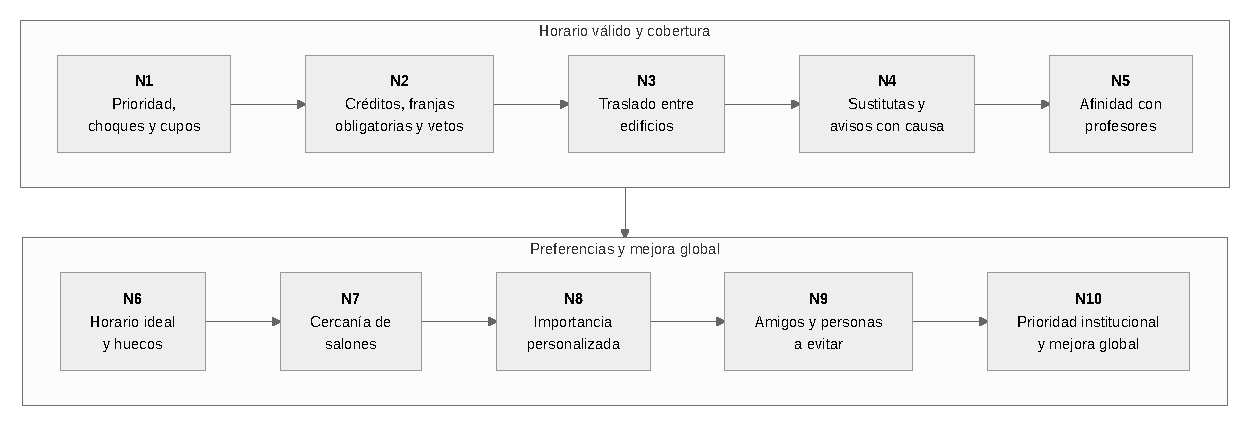
\includegraphics[width=\textwidth]{figuras/niveles.pdf}
\caption{Evolución del algoritmo. Los primeros niveles incorporan las reglas poco a poco; el horario final debe cumplir R1--R9.}\label{fig:niveles}
\end{figure}

\begin{table}[htbp]
\caption{Qué agrega cada nivel y cómo se comprueba}\label{tab:niveles}
\small
\begin{tabularx}{\textwidth}{@{}lLL@{}}
\toprule
Nivel & Qué agrega & Ejemplo de prueba \\
\midrule
N1 & Atiende las solicitudes de todos los estudiantes de mayor a menor prioridad y toma la primera sección con cupo que no choque (R1--R4) & Con cupo 1 y dos estudiantes, gana la solicitud de mayor prioridad \\
N2 & Tope de 20 créditos, franjas obligatorias y profesores vetados (R5--R7) & Quien trabaja el lunes de 14:00 a 20:00 no tiene clases en esa franja \\
N3 & Tiempo de traslado entre edificios (R8) & Clases seguidas en edificios a 15 minutos no son compatibles; a 8 minutos sí \\
N4 & Materias sustitutas (R9) y avisos con causa y sugerencia & Si la principal está llena y la sustituta cabe, queda la sustituta y se avisa \\
N5 & Entre las secciones válidas elige la que más satisface al estudiante; primer criterio: afinidad con profesores & Entre profesores con afinidad $+2$ y $-1$, elige el de $+2$ \\
N6 & Franjas preferidas, a evitar y libres deseables; pocos huecos & Quien prefiere mañanas queda en la sección de las 7:00 y no en la de las 18:00 \\
N7 & Cercanía entre salones & Con dos secciones iguales, elige la del edificio más cercano a la clase anterior \\
N8 & Importancia personal (alta, media o baja) de cada criterio & Invertir la importancia de profesores y horario cambia la sección elegida \\
N9 & Amigos y personas a evitar & Si se atienden las mismas materias, se favorece compartir sección \\
N10 & Desempate opcional por semestre y cambios de sección que mejoren el resultado según el orden definido & Un estudiante que en N9 quedó sin cupo lo obtiene cuando otro se mueve a una sección equivalente \\
\botrule
\end{tabularx}
\end{table}

Los niveles 1 a 9 ordenan las solicitudes y eligen para cada una la mejor sección disponible en ese momento. Una decisión temprana puede ocupar el último cupo que otro estudiante necesitaba. Por eso N10 revisa el conjunto de horarios e intenta mover estudiantes entre secciones.

Un cambio solo se acepta si cumple las reglas y mejora el resultado según la Sección~\ref{sec:objetivo}. Se fija un límite de cambios examinados y no se vuelve a una asignación peor o igual. Este procedimiento busca una buena respuesta, pero no garantiza la mejor posible. Se espera que el problema completo sea difícil de resolver de forma exacta, pues problemas cercanos, como la selección de intervalos por trabajos \cite{spieksma1999}, son NP-difíciles; aquí no se demuestra, y por eso la comparación exacta se limita a instancias pequeñas. Para medir qué tan cerca queda, se comparará con respuestas exactas en casos pequeños.

%%==================================================================%%
\section{Datos}\label{sec:datos}

\subsection{Formato y almacenamiento}

\begin{sloppypar}
Toda la información se guarda en archivos JSON dentro de la carpeta \texttt{data/} del proyecto, que funcionan como almacenamiento local: \texttt{materias.json}, \texttt{profesores.json}, \texttt{edificios.json}, \texttt{secciones.json}, \texttt{estudiantes.json} y, de forma opcional, \texttt{config.json}. Cada corrida guarda su salida en \texttt{resultados/}. Para cambiar los datos basta con editar los archivos, importarlos desde la aplicación o usar sus formularios, que escriben en los mismos archivos. Un ejemplo de sección y de estudiante:
\end{sloppypar}

\begin{minipage}{\textwidth}
\begin{lstlisting}[style=json]
{ "id": "CAL1-02", "materia": "CAL1", "profesor": "p12", "cupo": 30,
  "sesiones": [ { "dia": "L", "inicio": "07:00", "fin": "09:00", "edificio": "A", "salon": "A-201" },
                { "dia": "X", "inicio": "07:00", "fin": "09:00", "edificio": "A", "salon": "A-201" } ] }
\end{lstlisting}
\end{minipage}


\begin{minipage}{\textwidth}
\begin{lstlisting}[style=json]
{ "id": "e001", "nombre": "Laura Gómez", "semestre": 5,
  "materias": [ { "codigo": "CAL1", "prioridad": 5, "sustitutas": ["CAL2"] },
                { "codigo": "FIS1", "prioridad": 3 } ],
  "franjas_libres": [ { "dia": "L", "inicio": "14:00", "fin": "20:00", "tipo": "obligatoria" },
                      { "dia": "*", "inicio": "13:00", "fin": "14:00", "tipo": "deseable" } ],
  "franjas_preferidas": [ { "dia": "*", "inicio": "09:00", "fin": "13:00" } ],
  "franjas_evitadas":   [ { "dia": "*", "inicio": "07:00", "fin": "08:00" } ],
  "profesores": [ { "id": "p12", "afinidad": 2 }, { "id": "p40", "veto": true } ],
  "social": [ { "estudiante": "e017", "afinidad": 2 }, { "estudiante": "e090", "afinidad": -2 } ],
  "importancia": { "horario": "media", "profesores": "alta", "cercania": "media",
                   "huecos": "baja", "social": "alta" } }
\end{lstlisting}
\end{minipage}


La salida contiene, por estudiante, sus secciones, sus avisos y su satisfacción, y un resumen general:

Este fragmento muestra cómo se registra la respuesta a cada solicitud. Es un ejemplo del formato; los porcentajes y puntajes se calculan sobre el resultado completo como se explica en la Sección~\ref{sec:metricas}.

\begin{minipage}{\textwidth}
\begin{lstlisting}[style=json]
{ "id": "e001",
  "solicitudes": [
    { "materia": "CAL1", "estado": "principal", "seccion": "CAL1-02" },
    { "materia": "FIS1", "estado": "no_inscrita", "seccion": null }
  ],
  "avisos": [ { "materia": "FIS1", "causa": "Cupo lleno",
                "sugerencia": "Revisar alternativas y oferta de cupos" } ] }
\end{lstlisting}
\end{minipage}


\subsection{Generación de datos y respuestas esperadas}

Los JSON siguen RFC~8259 \cite{json}. Además de los archivos anteriores, \texttt{traslados.json} guarda origen, destino y minutos para cada par de edificios. Cada prueba conserva sus entradas, parámetros y versiones del generador y del algoritmo. Si no hay \texttt{config.json}, se usan 20 créditos, sustitución de 0,8, semestre desactivado, semilla 42 y hasta 10.000 cambios examinados en la mejora.

Se crearán dos tipos de datos, siempre con nombres y códigos ficticios:
\begin{enumerate}
\item \textbf{Escenarios variados.} Se generan materias, profesores, edificios y traslados; después, secciones con horarios, salones y cupos válidos; finalmente, estudiantes, solicitudes y preferencias con códigos existentes. Si una sesión cruza un profesor o salón, se prueba otra opción hasta un límite de intentos. Para variar la dificultad se ajustan cupos, demanda, prioridades, proporción de estudiantes que trabajan, sustitutas, vetos y preferencias sobre compañeros.
\item \textbf{Casos con respuesta conocida.} Se parte de horarios válidos para todos los estudiantes a la vez, respetando cupos y demás reglas. De ellos se obtienen las solicitudes principales y se agregan secciones alternativas. La asignación inicial se guarda como referencia: demuestra que todas las materias caben, aunque otra respuesta podría satisfacer mejor las preferencias.
\end{enumerate}

La semilla permite repetir las elecciones del generador si también se conservan sus parámetros y versión. En casos muy pequeños se revisan todas las combinaciones válidas o se usa CP-SAT de OR-Tools \cite{cpsat}, respetando el orden de prioridades de la Sección~\ref{sec:objetivo}. Solo se llama óptima a una respuesta si se comprueba que no existe otra mejor. Cada caso guarda la entrada y la respuesta esperada; si hay empates, se guardan los puntajes y las condiciones que deben cumplir las respuestas aceptables.

\paragraph{Ejemplo completo de una prueba pequeña.}
Se crean una materia M1 de tres créditos, un profesor P1 y un edificio B1. M1 tiene una sola sección, S1, con un cupo y una sesión el lunes de 07:00 a 09:00 en B1. Dos estudiantes, e01 de segundo semestre y e02 de octavo, solicitan M1 con prioridad 5. No tienen sustitutas ni preferencias. El traslado de B1 a B1 es cero y el límite de créditos es 20. Con desempate por semestre activado, se espera S1 para e02, tres créditos para él y un aviso de no inscripción para e01. Desactivado, se espera S1 para e01 por el desempate final de códigos. En ambos casos se atiende una solicitud de prioridad 5 y no se incumple ninguna regla.

\begin{table}[htbp]
\caption{Casos de prueba y resultados esperados.}\label{tab:aceptacion}
\small
\begin{tabularx}{\textwidth}{@{}lLL@{}}
\toprule
Caso & Datos de la prueba & Resultado esperado \\
\midrule
Prioridades & Una solicitud de prioridad 5 impide dos de prioridad 1 & Se conserva la de prioridad 5 \\
Semestre & Dos solicitudes iguales, un cupo; semestres 2 y 8 & Activado: gana semestre 8; desactivado: decide el código si todo lo demás es igual \\
Límite del semestre & Prioridad 5 en semestre 2 y prioridad 4 en semestre 8, un cupo & Gana la de prioridad 5 en ambas configuraciones \\
Preferencias & Elegir el profesor preferido hace perder una solicitud de prioridad 5 & Se conserva la mayor atención de prioridad 5 \\
Traslado & Clases seguidas, edificios a 10 u 11 minutos & A 10 es posible; a 11 no \\
Créditos & Alternativas que llevan a 20 o 21 créditos & 20 permitido; 21 descartado \\
Sustitución & Principal sin secciones, sustituta compatible & Se inscribe la sustituta, aporta 0,8 y se genera un aviso \\
No duplicación & Una sustituta común a dos solicitudes & Una inscripción atiende como máximo una solicitud \\
Solicitud vacía & Estudiante sin solicitudes & Horario vacío y sin avisos \\
Datos incorrectos & Sección con profesor inexistente & Se informa el error y no se ejecuta \\
\botrule
\end{tabularx}
\end{table}

\subsection{Evaluación y comprobación}

Se probarán 20, 200, 500 y 2.000 estudiantes, con cupos suficientes, ajustados y escasos y diez semillas por escenario (0 a 9). Los casos exactos serán menores: de 2 a 6 estudiantes, de 1 a 3 solicitudes por estudiante y de 1 a 2 secciones por materia.

Se comparará con una asignación aleatoria válida y otra por orden de llegada, usando los mismos datos y reglas. Se medirán materias atendidas por prioridad, principales y sustituciones, satisfacción promedio y mínima, reglas incumplidas y tiempo del algoritmo. La lectura de datos y la verificación se miden aparte. Se registran equipo y versiones y se resumen mediana y rango entre semillas.

Se mantienen casos pequeños por nivel, casos con respuesta conocida y casos límite de la Tabla~\ref{tab:aceptacion}. El verificador también recibirá respuestas con errores intencionales, como exceso de cupo o materias duplicadas. Reordenar los registros de entrada sin cambiar sus datos no debe cambiar el resultado. Los niveles con reglas distintas se comparan indicando esa diferencia. Las pruebas se ejecutarán durante la implementación; aquí se presenta su diseño.


%%==================================================================%%
\section{Tecnología y arquitectura}\label{sec:tec}

\begin{table}[htbp]
\caption{Tecnología del proyecto}\label{tab:tec}
\small
\begin{tabularx}{\textwidth}{@{}lL@{}}
\toprule
Parte & Tecnología \\
\midrule
Algoritmo & Python, como un módulo independiente de la web \\
Servidor & FastAPI, que lee y escribe los JSON y lanza las corridas \\
Aplicación web & React con TypeScript \\
Datos & Archivos JSON locales, validados al cargarlos \\
Solver de comparación & OR-Tools CP-SAT, solo para instancias pequeñas \\
Pruebas y versiones & pytest, Git y GitHub con integración continua \\
Despliegue & Primero local; después Docker Compose \\
Documentación & \LaTeX\ y diagramas en Mermaid \\
\botrule
\end{tabularx}
\end{table}

La aplicación web habla con el servidor, el servidor lee y guarda los archivos JSON y llama al algoritmo, y el verificador revisa cada resultado (Figura~\ref{fig:arq}). El despliegue se hará en dos fases: primero, el servidor y la web se ejecutan localmente en el computador de desarrollo; después, una vez estable, se empaquetan con Docker Compose en dos contenedores, manteniendo la carpeta \texttt{data/} fuera del contenedor para que los JSON se sigan editando directamente.

\begin{figure}[H]
\centering
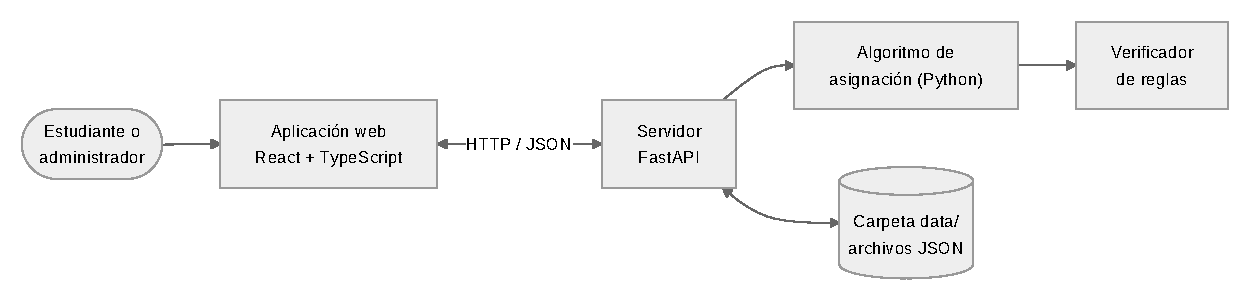
\includegraphics[width=0.9\textwidth]{figuras/arquitectura.pdf}
\caption{Arquitectura general.}\label{fig:arq}
\end{figure}

%%==================================================================%%
\section{Interfaz y flujo de uso}\label{sec:ui}

La aplicación permite cargar datos, indicar preferencias y consultar los horarios. Se elige al estudiante mediante un selector, sin iniciar sesión. El recorrido es \emph{Datos, Estudiantes, Preferencias, Ejecutar, Resultados y Horario}:
\begin{enumerate}
\item \textbf{Datos y estudiantes.} Se importan los JSON o se generan datos de prueba. Los errores impiden ejecutar; una demanda superior a los cupos solo genera una advertencia. Se permite guardar una copia antes de reemplazar los datos.
\item \textbf{Preferencias.} Se buscan estudiantes por nombre o código y se editan materias, prioridades, sustitutas, franjas, profesores y compañeros. Guardar valida los cambios; cancelar conserva la información anterior.
\item \textbf{Ejecución.} Se elige el nivel y, en N10, se puede activar el desempate por semestre. Se recuerdan las prioridades de decisión, se calcula la asignación y se verifican las reglas. Los niveles incompletos se identifican como pruebas.
\item \textbf{Resultados y horario.} Se consultan materias atendidas, satisfacción, avisos y tiempo; se puede descargar la salida con los datos usados. El horario muestra las clases semanales y sus sustituciones. Editar preferencias y ejecutar de nuevo conserva el resultado anterior.
\end{enumerate}

La Figura~\ref{fig:ui-flujo} resume el recorrido completo y las Figuras~\ref{fig:ui-datos} a~\ref{fig:ui-horario} muestran cada pantalla: preparar los datos, elegir al estudiante, indicar las preferencias, ejecutar la asignación, revisar los resultados globales y consultar el horario. Los valores de las pantallas son ilustrativos, no resultados de pruebas.

\begin{figure}[htbp]
\centering
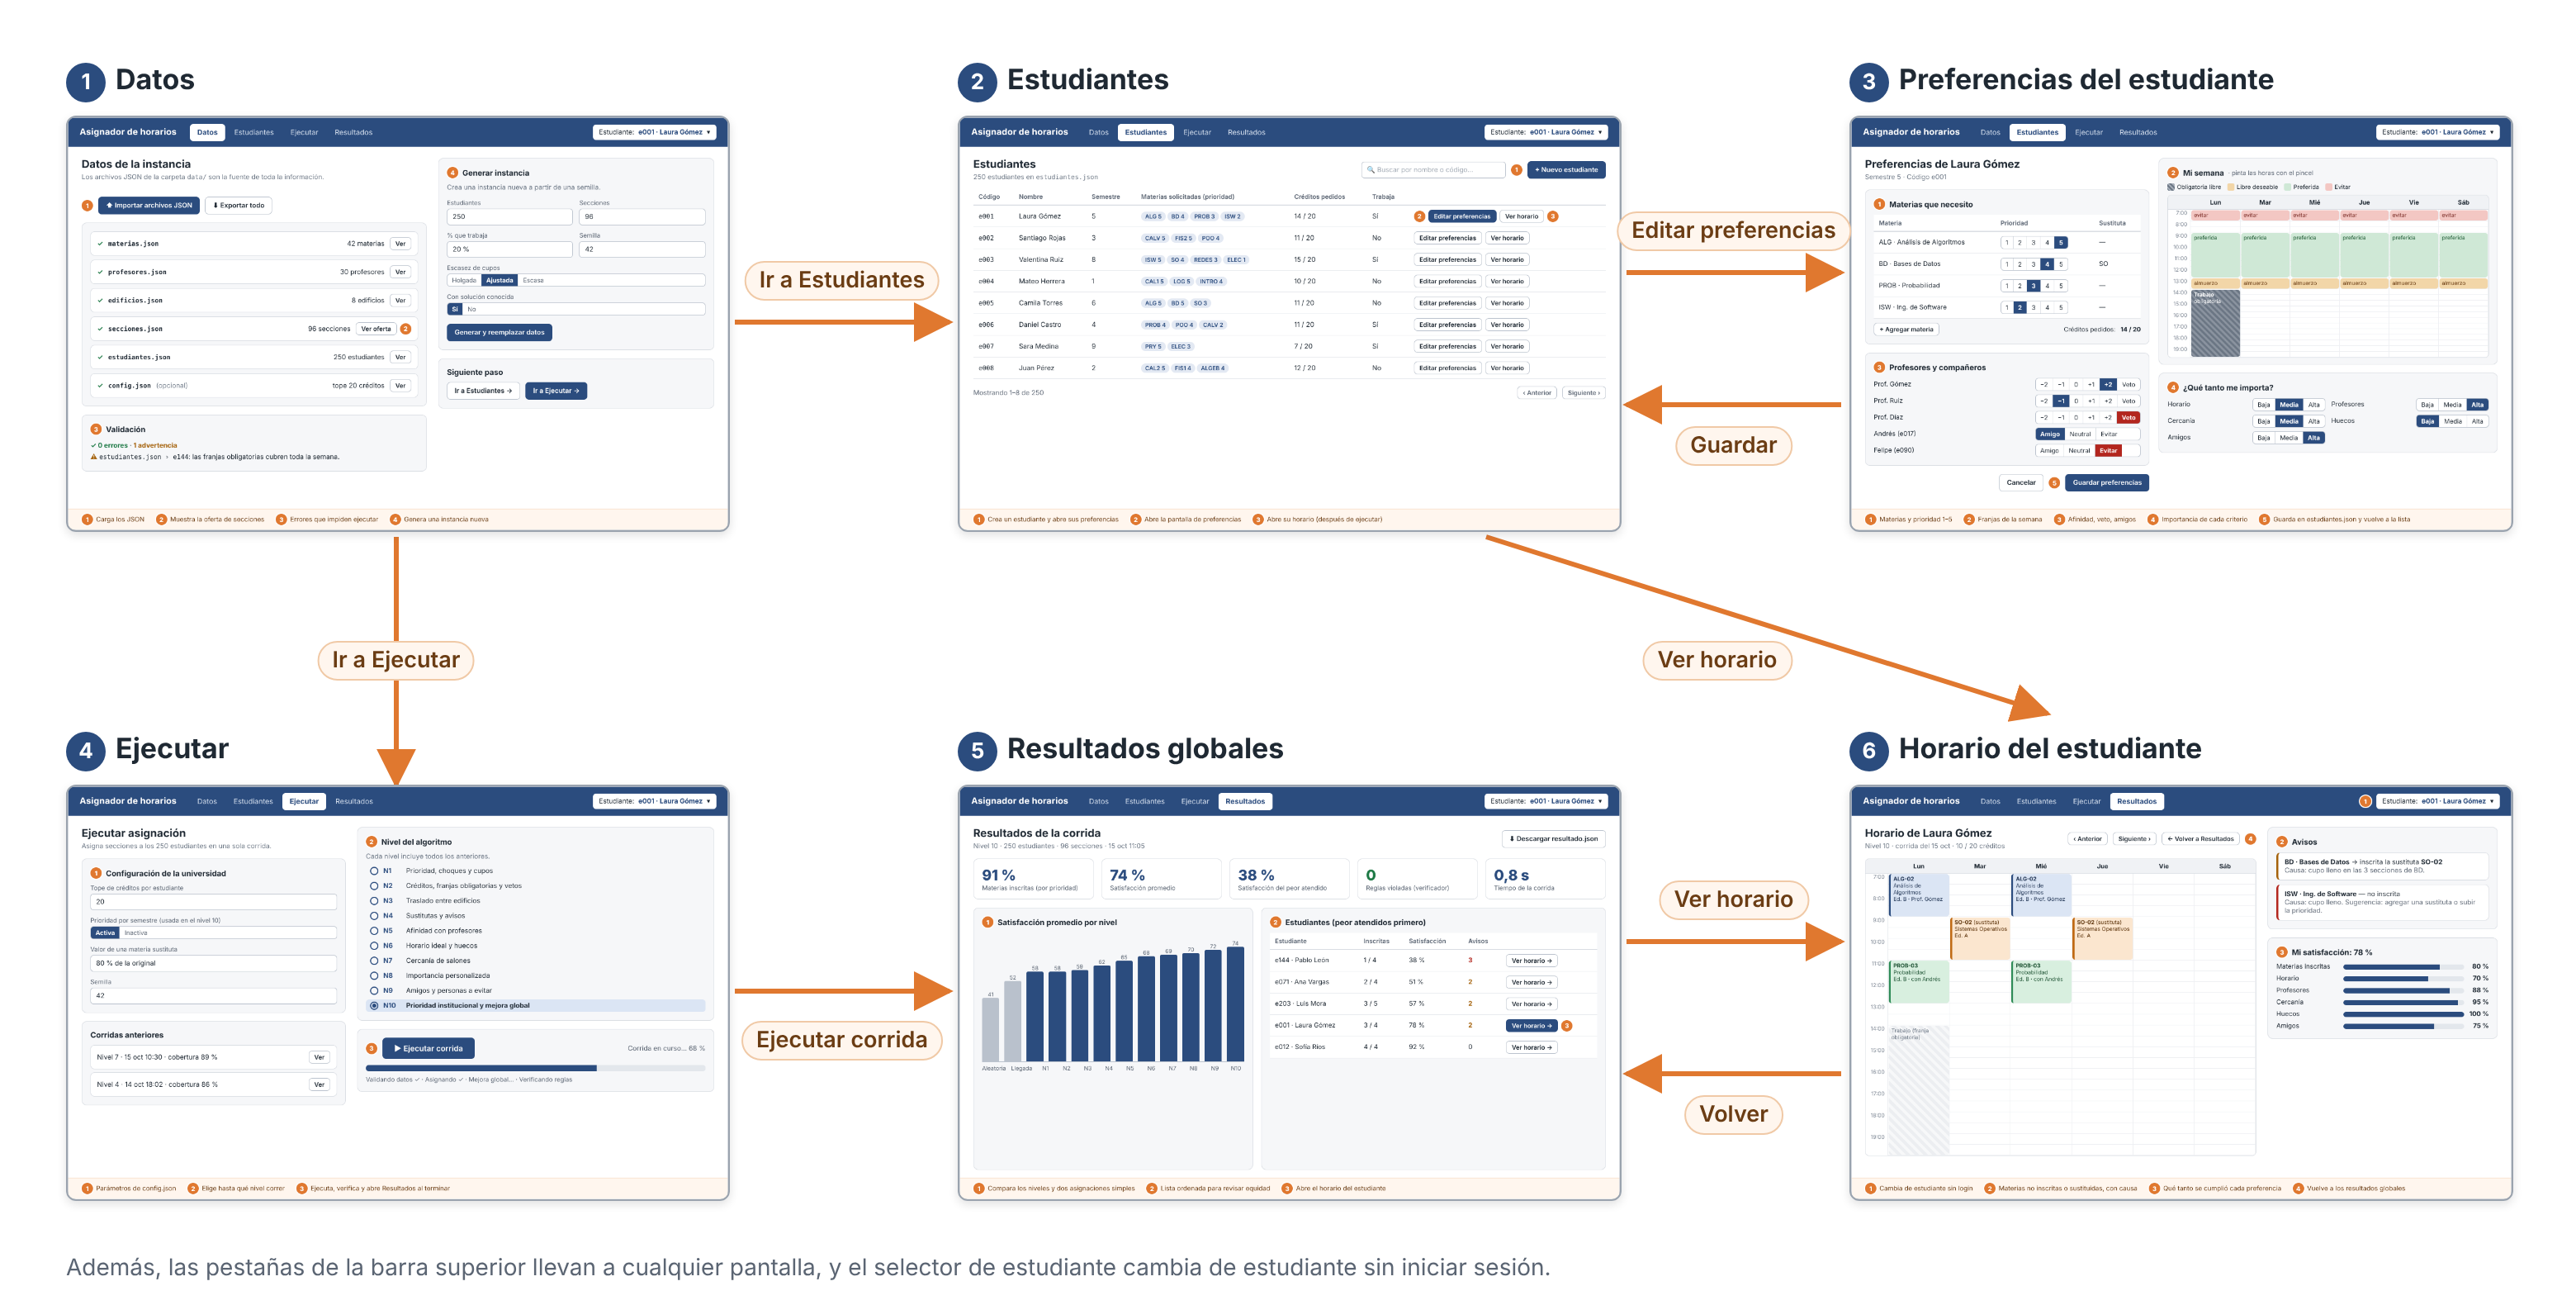
\includegraphics[width=\textwidth]{figuras/mockup_flujo.png}
\caption{Flujo general de la aplicación: seis pantallas y las acciones que llevan de una a otra.}\label{fig:ui-flujo}
\end{figure}

\begin{figure}[htbp]
\centering
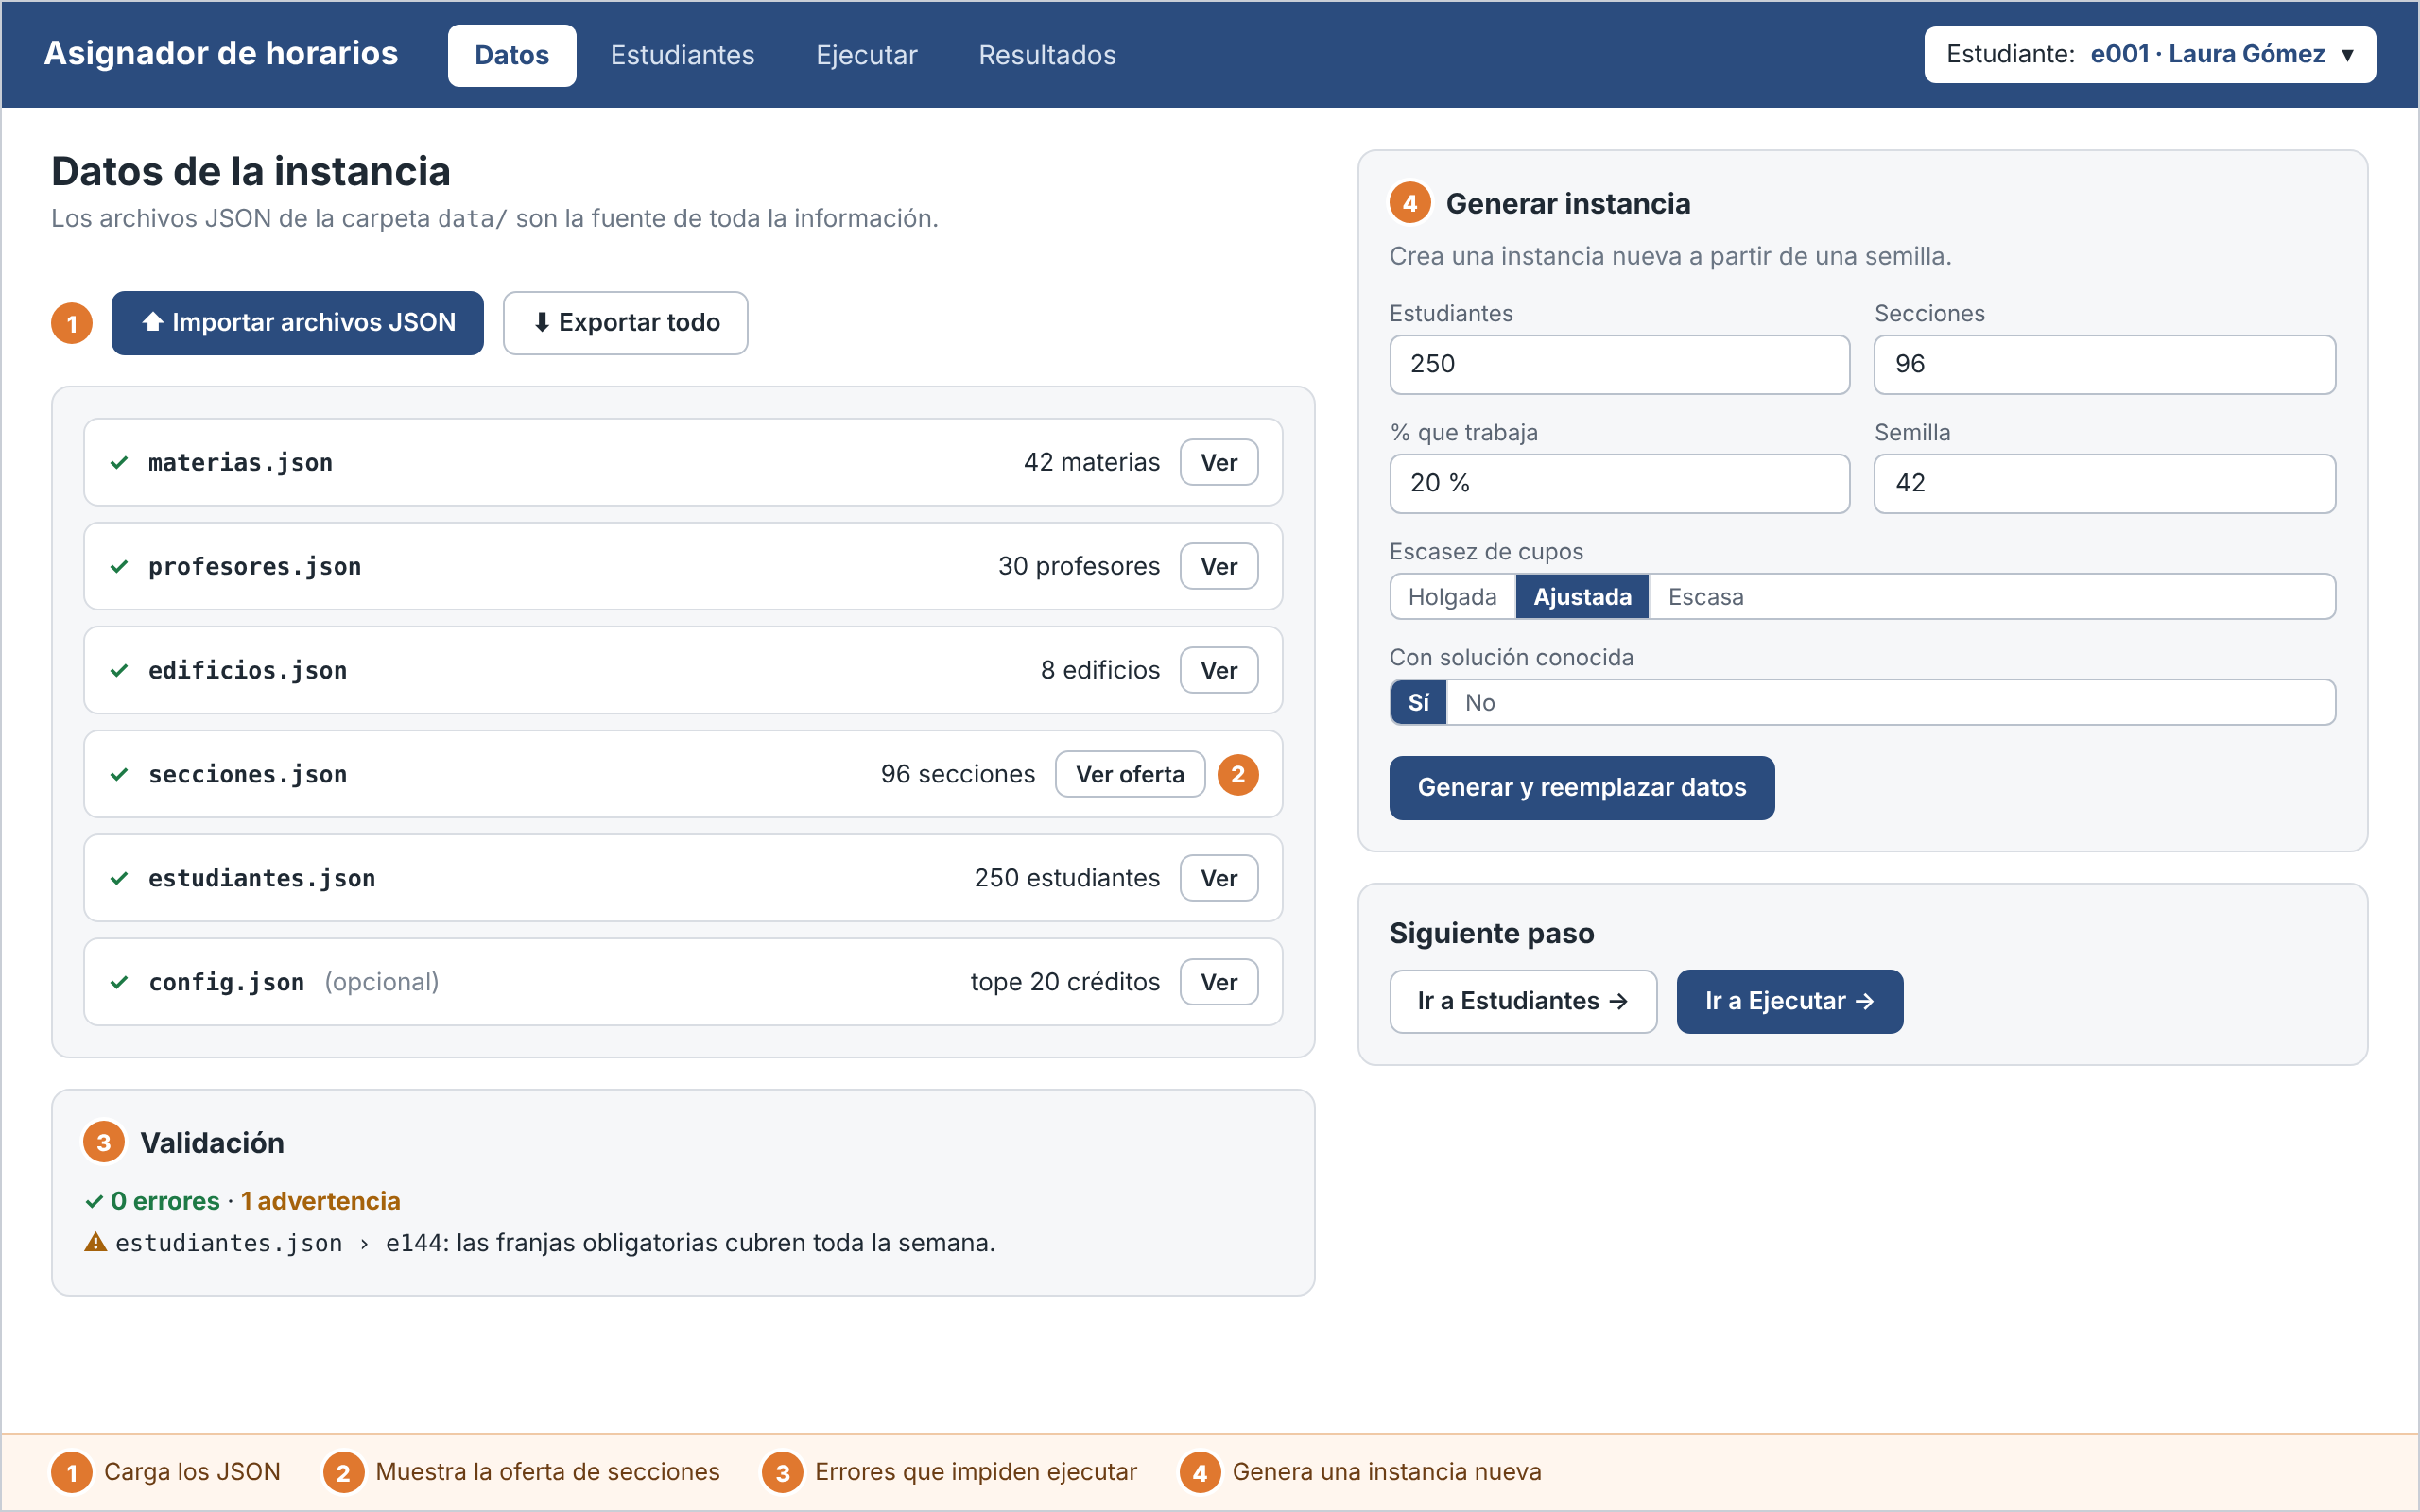
\includegraphics[width=\textwidth]{figuras/mockup1_datos.png}
\caption{Carga de archivos, generación de datos de prueba y revisión de errores.}\label{fig:ui-datos}
\end{figure}

\begin{figure}[htbp]
\centering
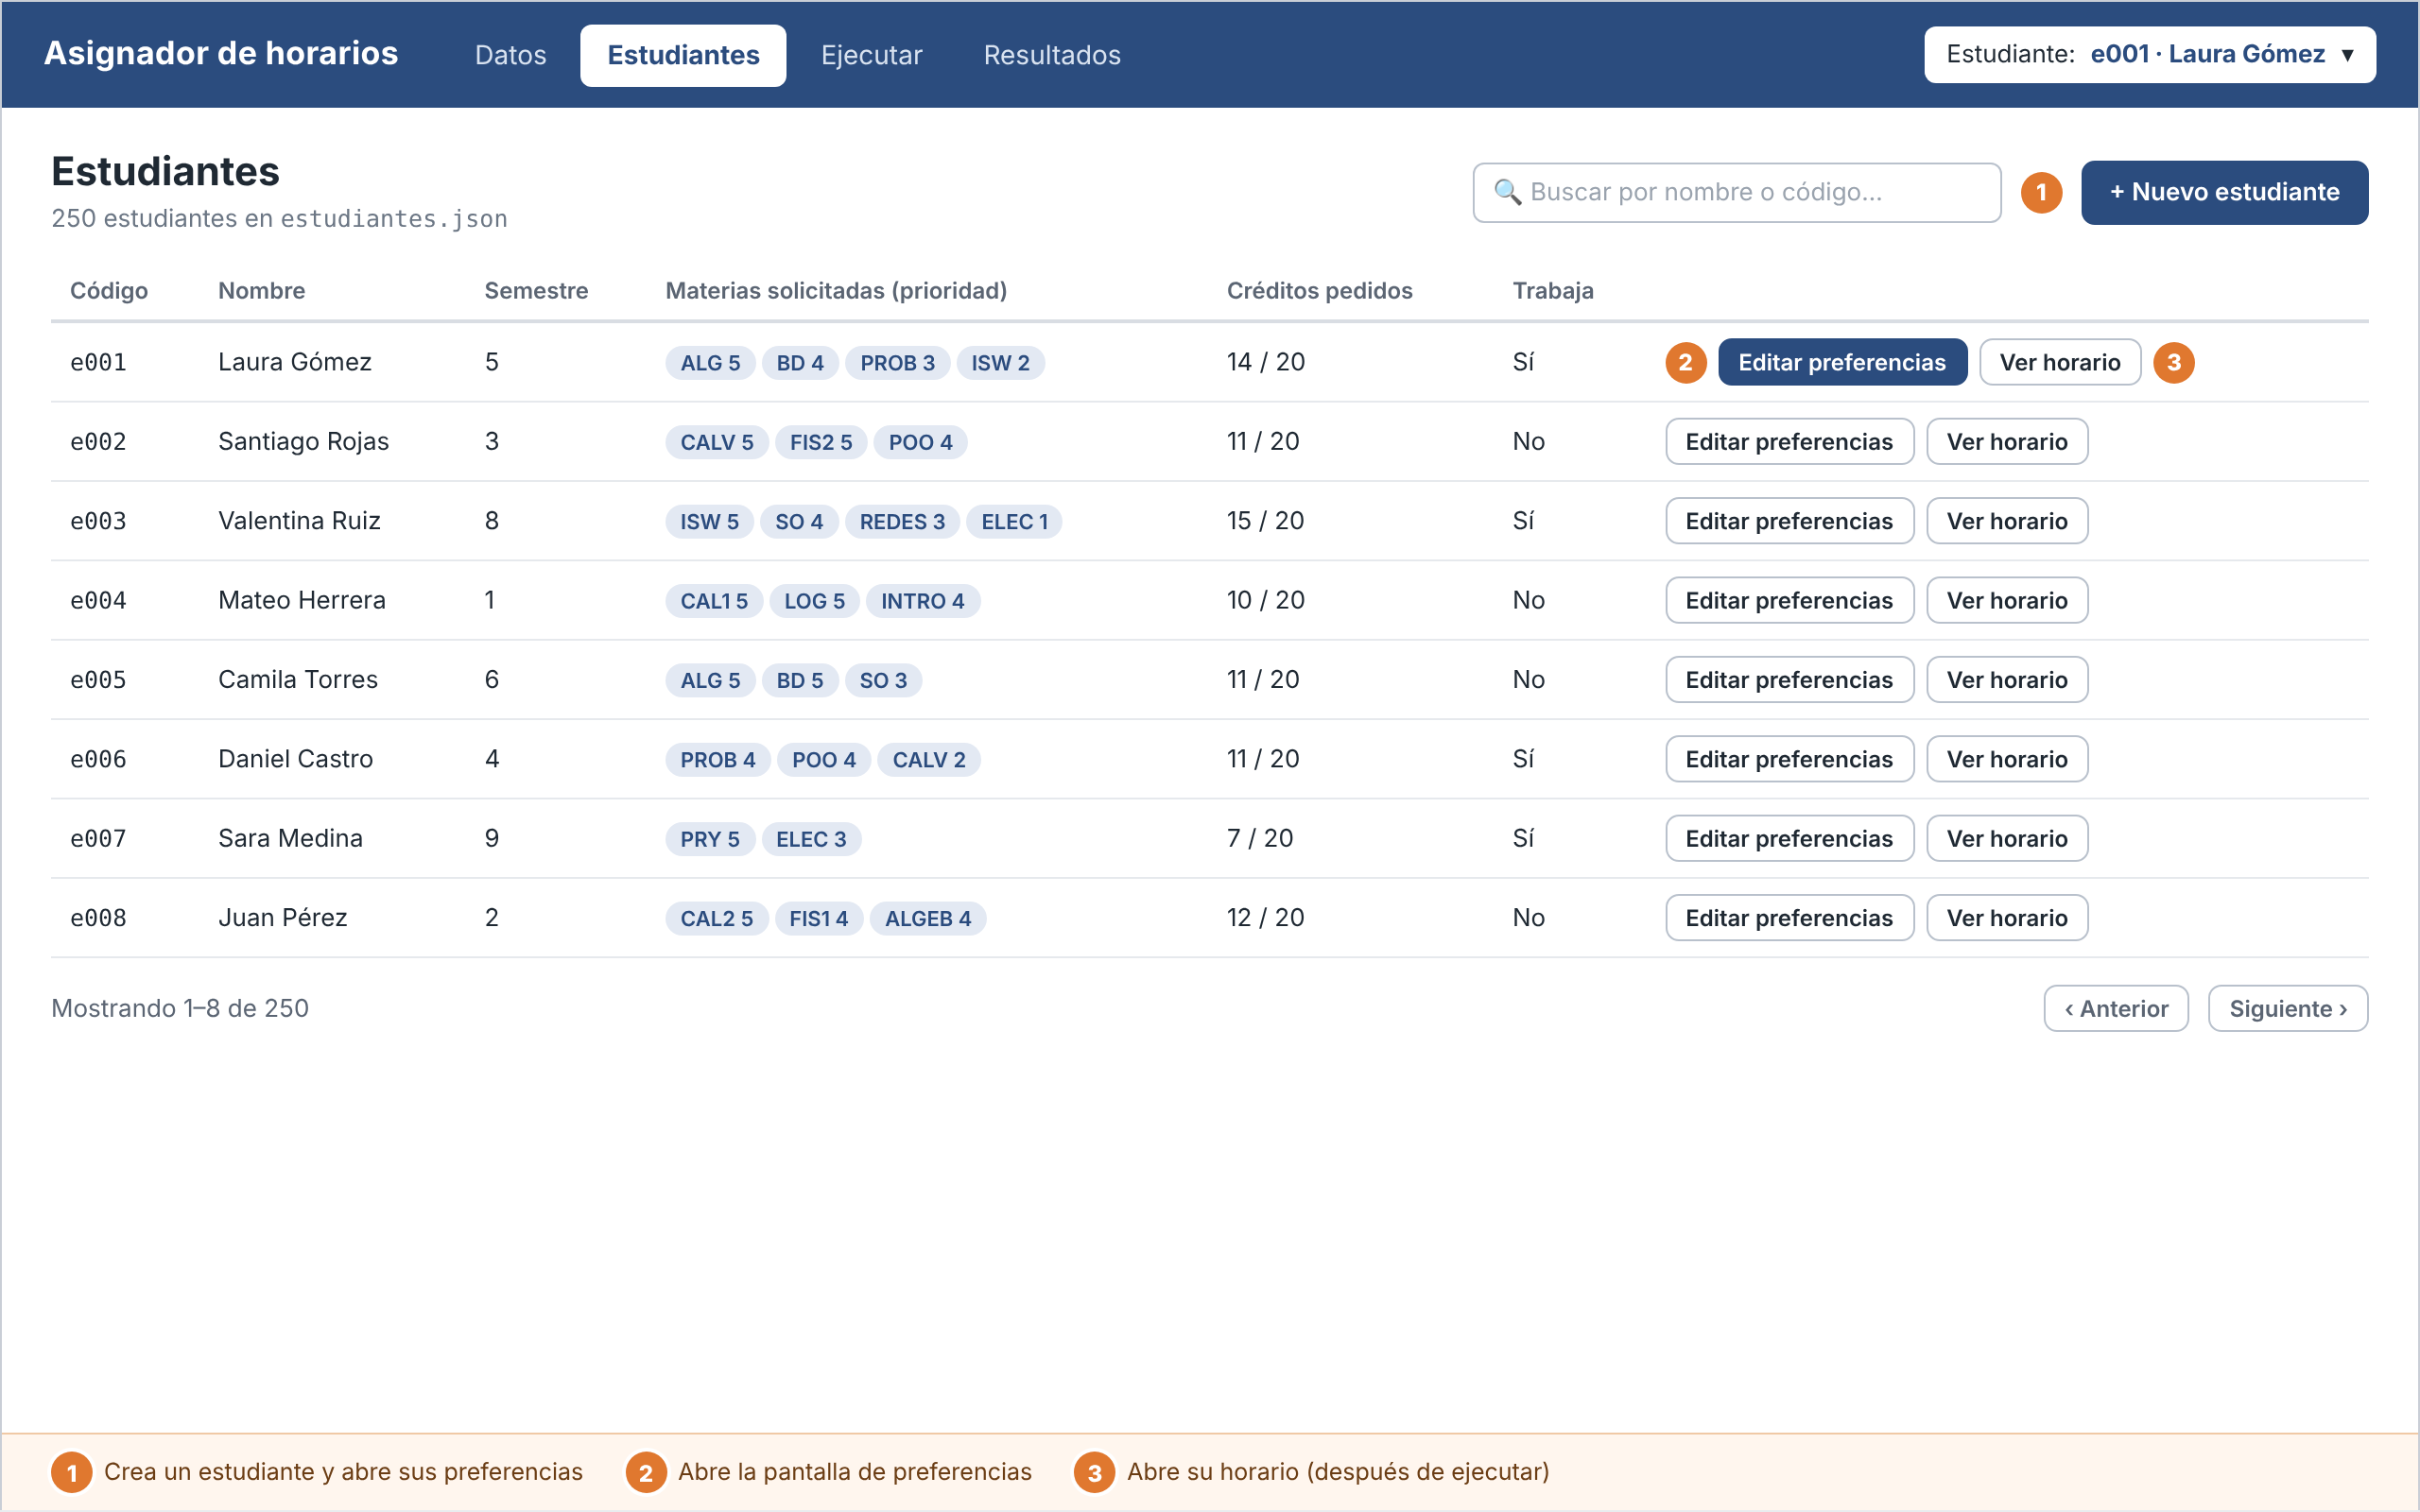
\includegraphics[width=\textwidth]{figuras/mockup2_estudiantes.png}
\caption{Lista de estudiantes con sus materias, prioridades y créditos pedidos.}\label{fig:ui-estudiantes}
\end{figure}

\begin{figure}[htbp]
\centering
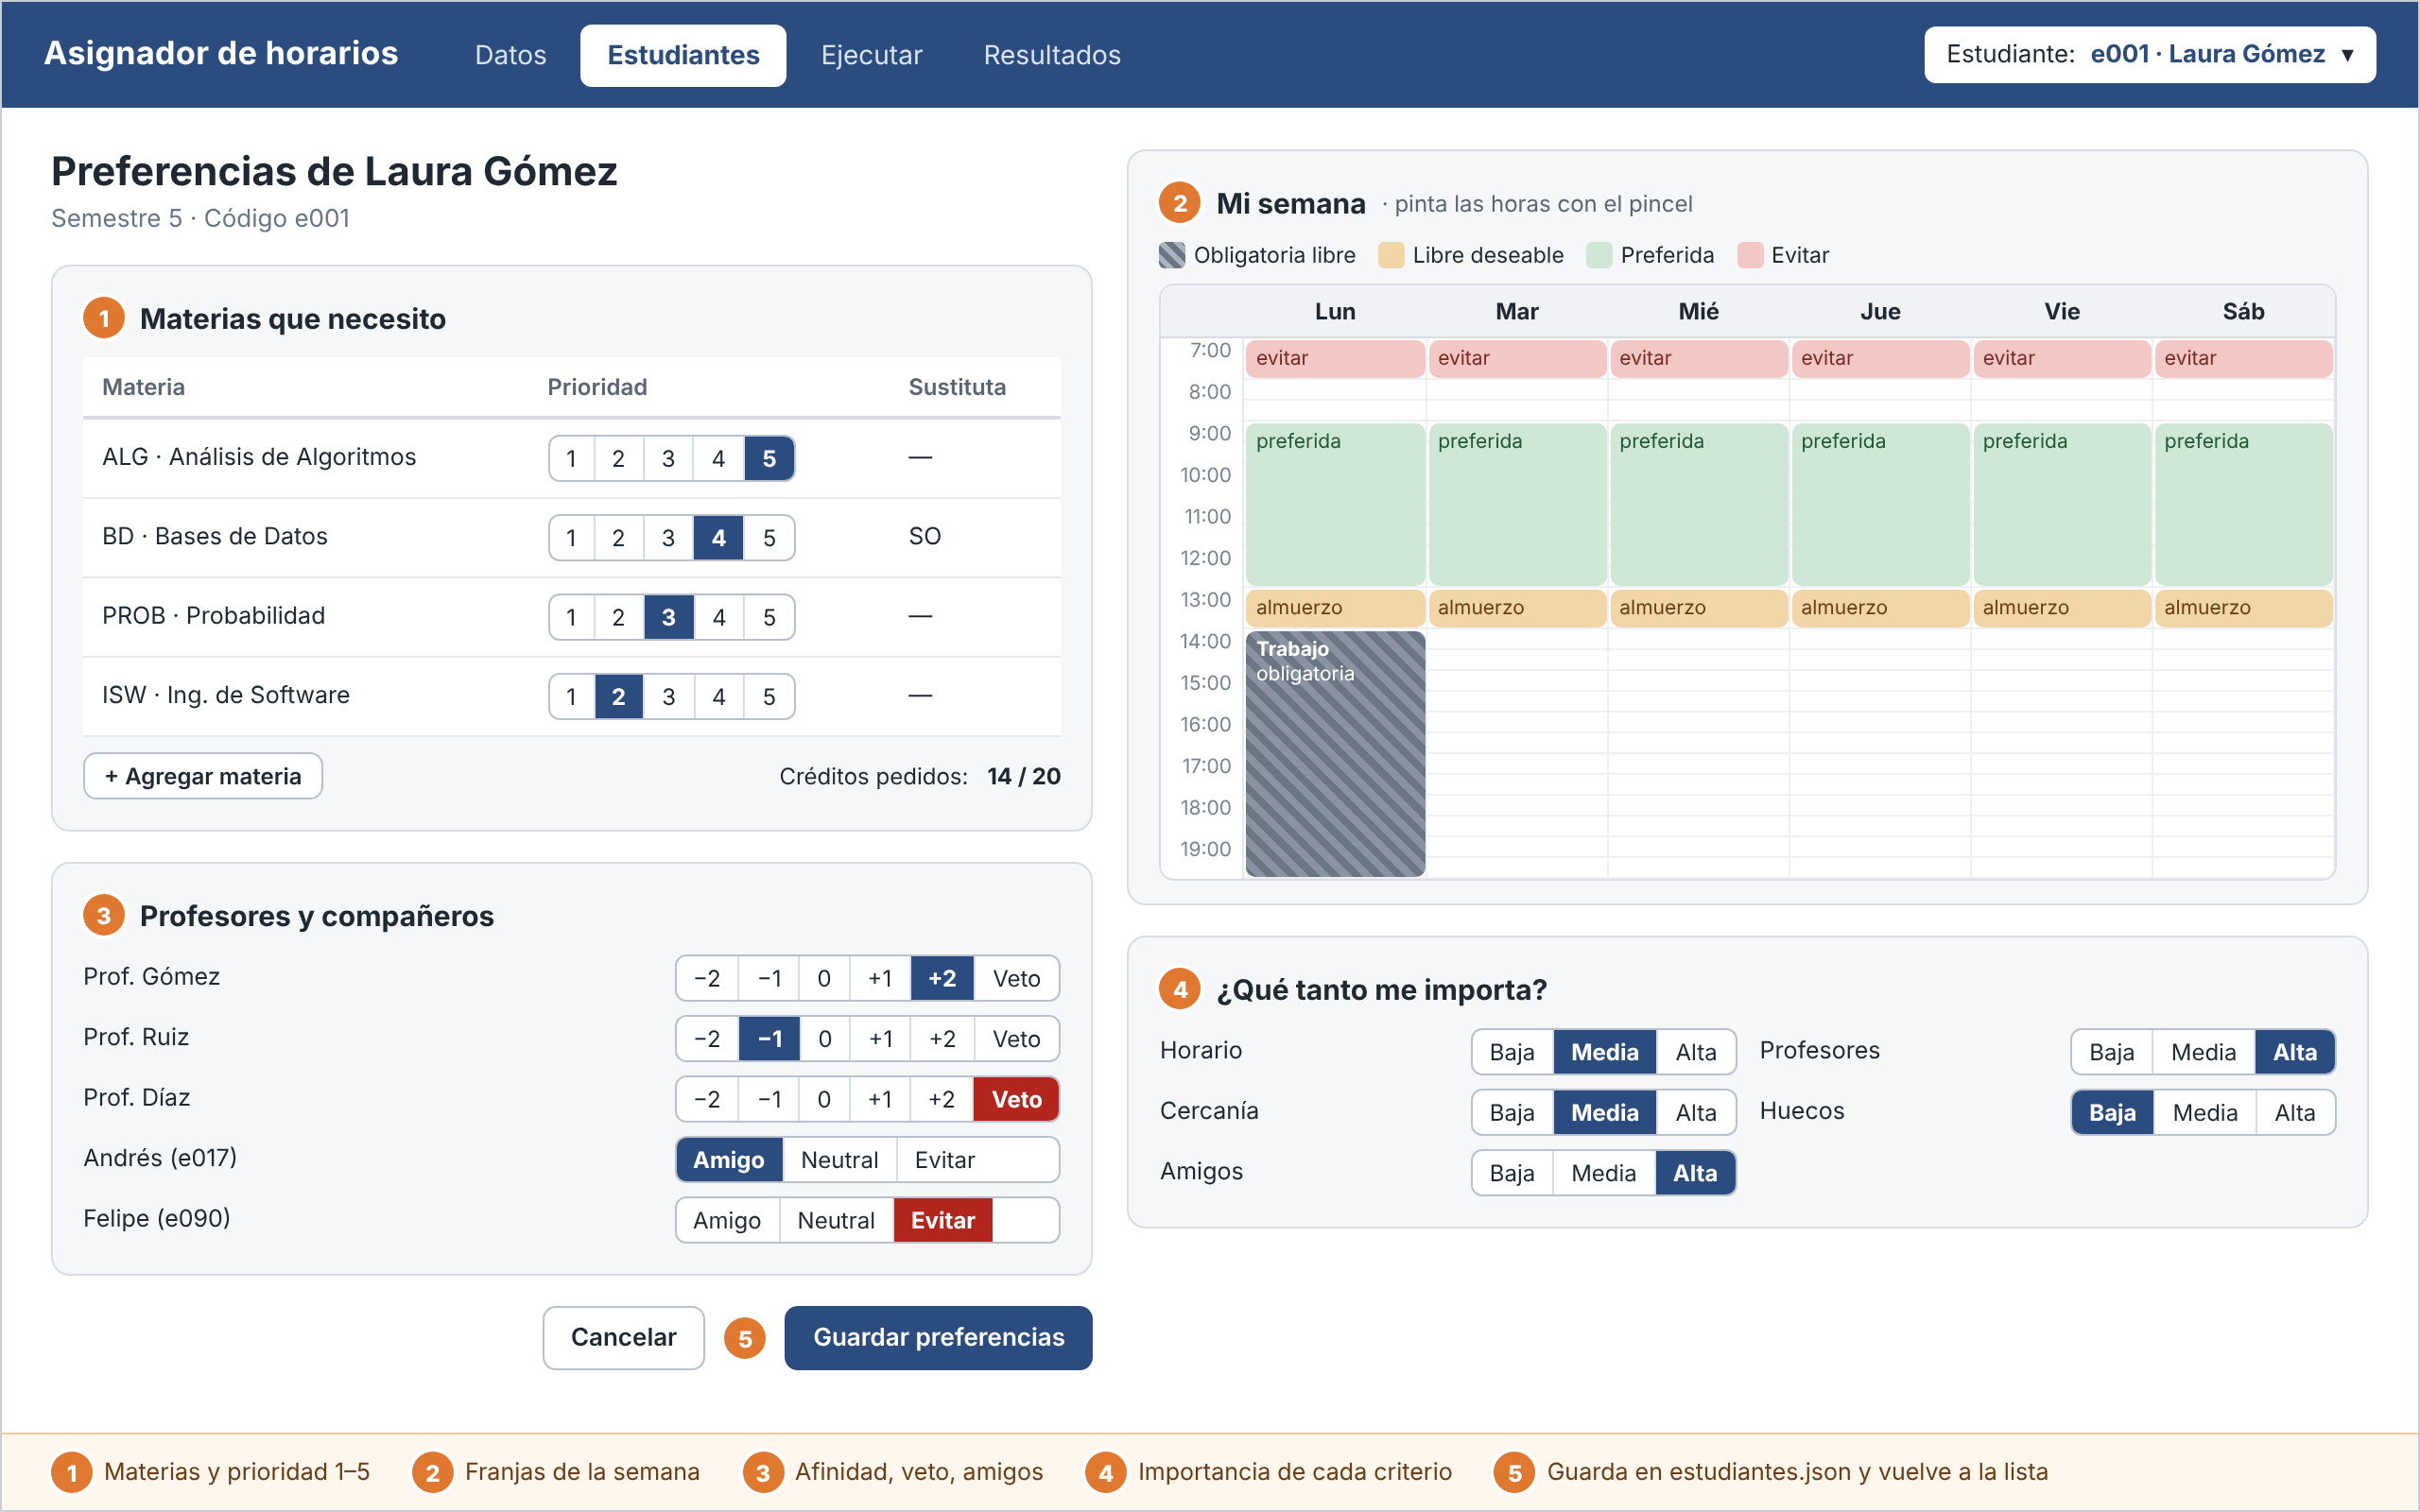
\includegraphics[width=\textwidth]{figuras/mockup3_preferencias.png}
\caption{Selección de materias y prioridades, franjas horarias, profesores y compañeros.}\label{fig:ui-preferencias}
\end{figure}

\begin{figure}[htbp]
\centering
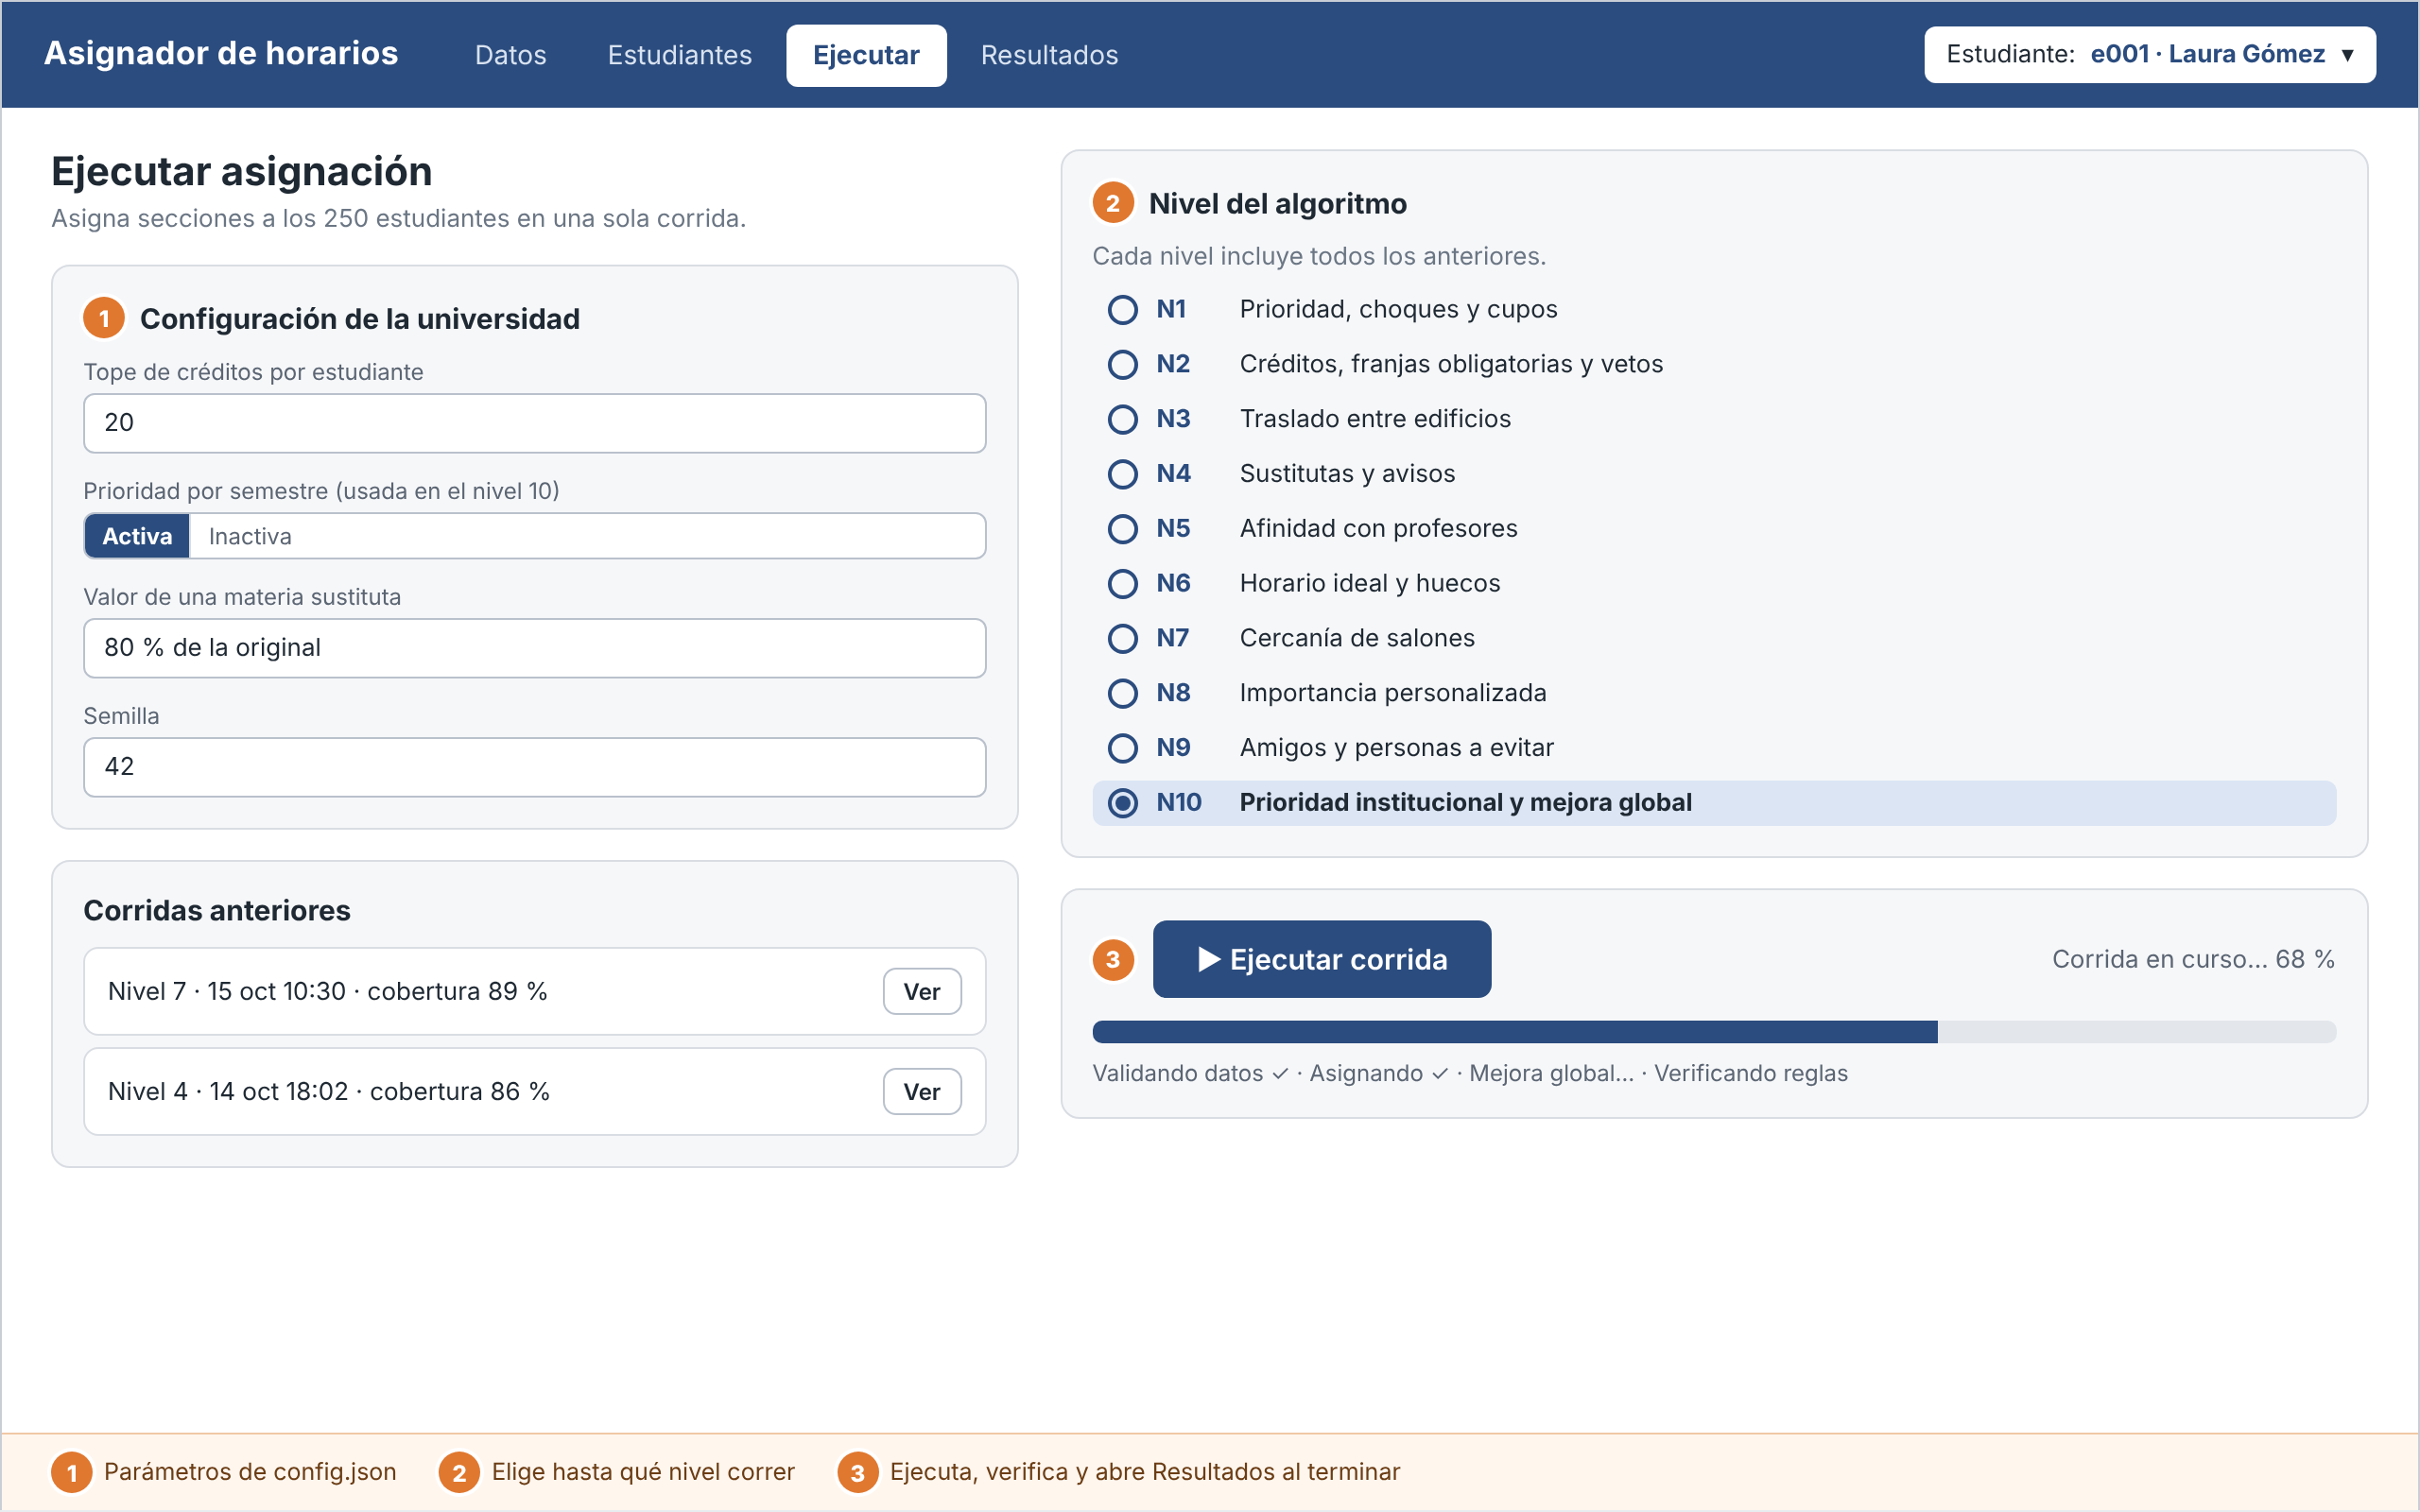
\includegraphics[width=\textwidth]{figuras/mockup4_ejecutar.png}
\caption{Configuración de la universidad, elección del nivel del algoritmo y ejecución de la corrida.}\label{fig:ui-ejecutar}
\end{figure}

\begin{figure}[htbp]
\centering
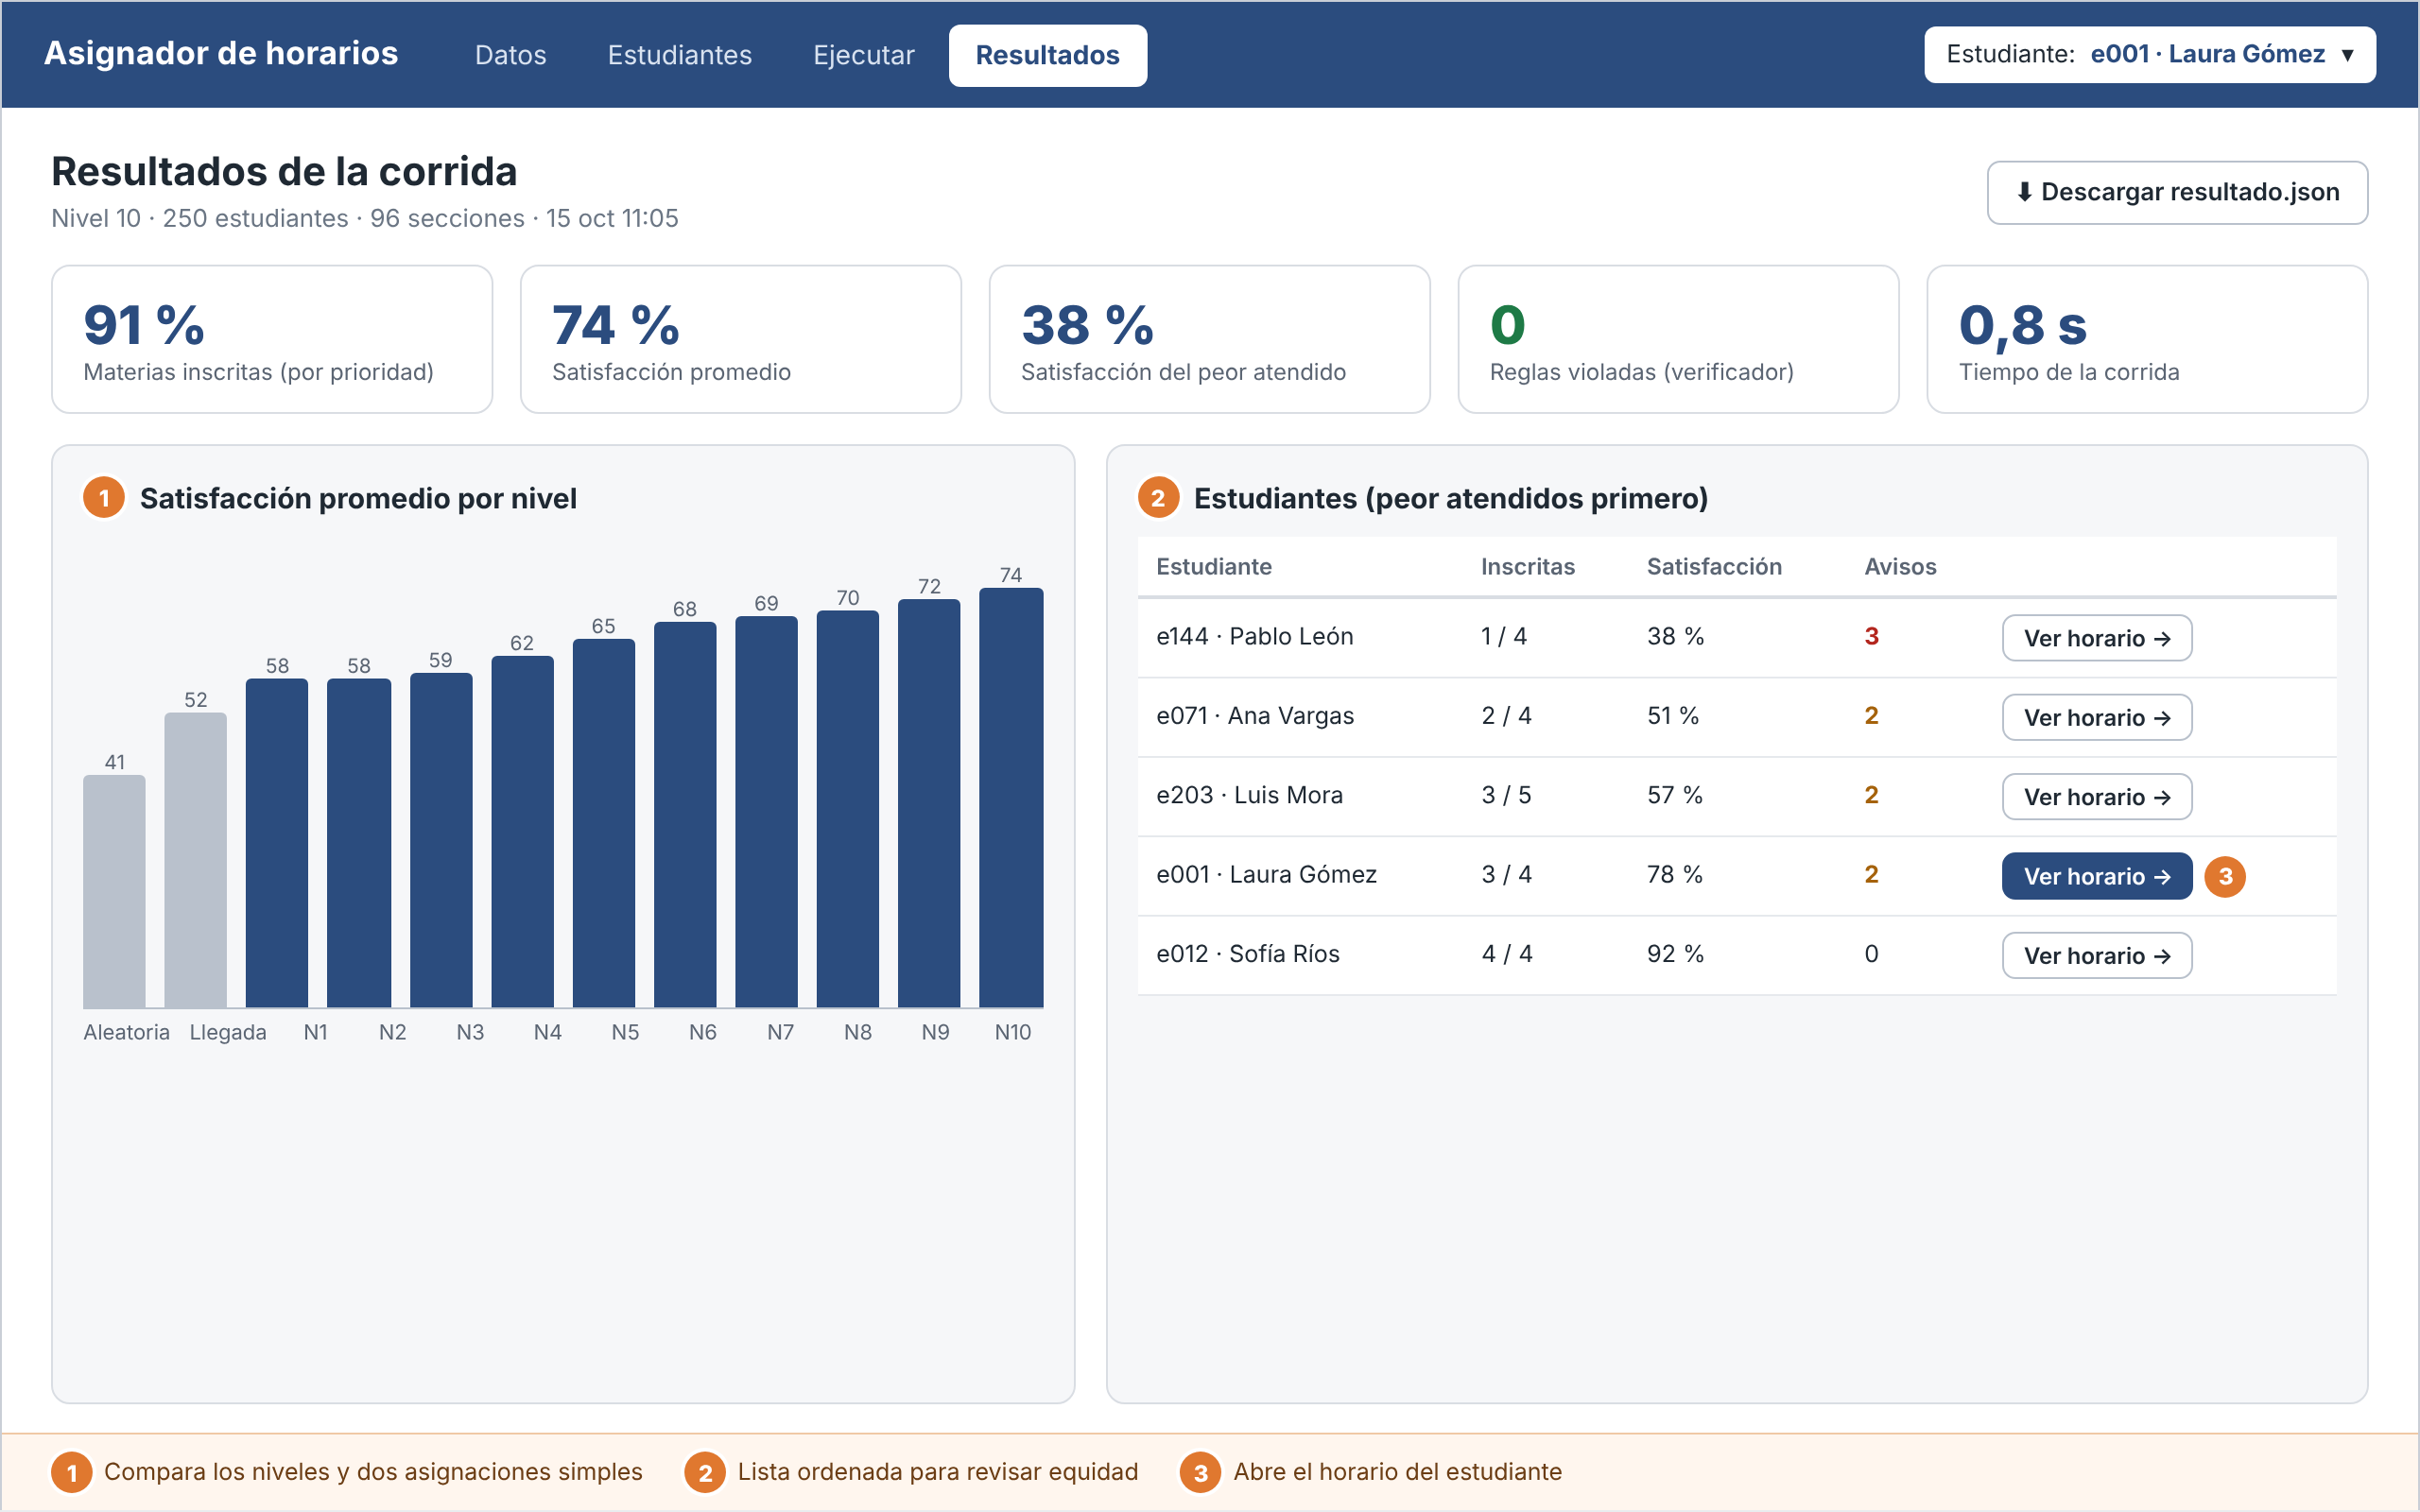
\includegraphics[width=\textwidth]{figuras/mockup5_resultados.png}
\caption{Resultados globales: indicadores de la corrida, comparación entre niveles y estudiantes peor atendidos.}\label{fig:ui-resultados}
\end{figure}

\begin{figure}[htbp]
\centering
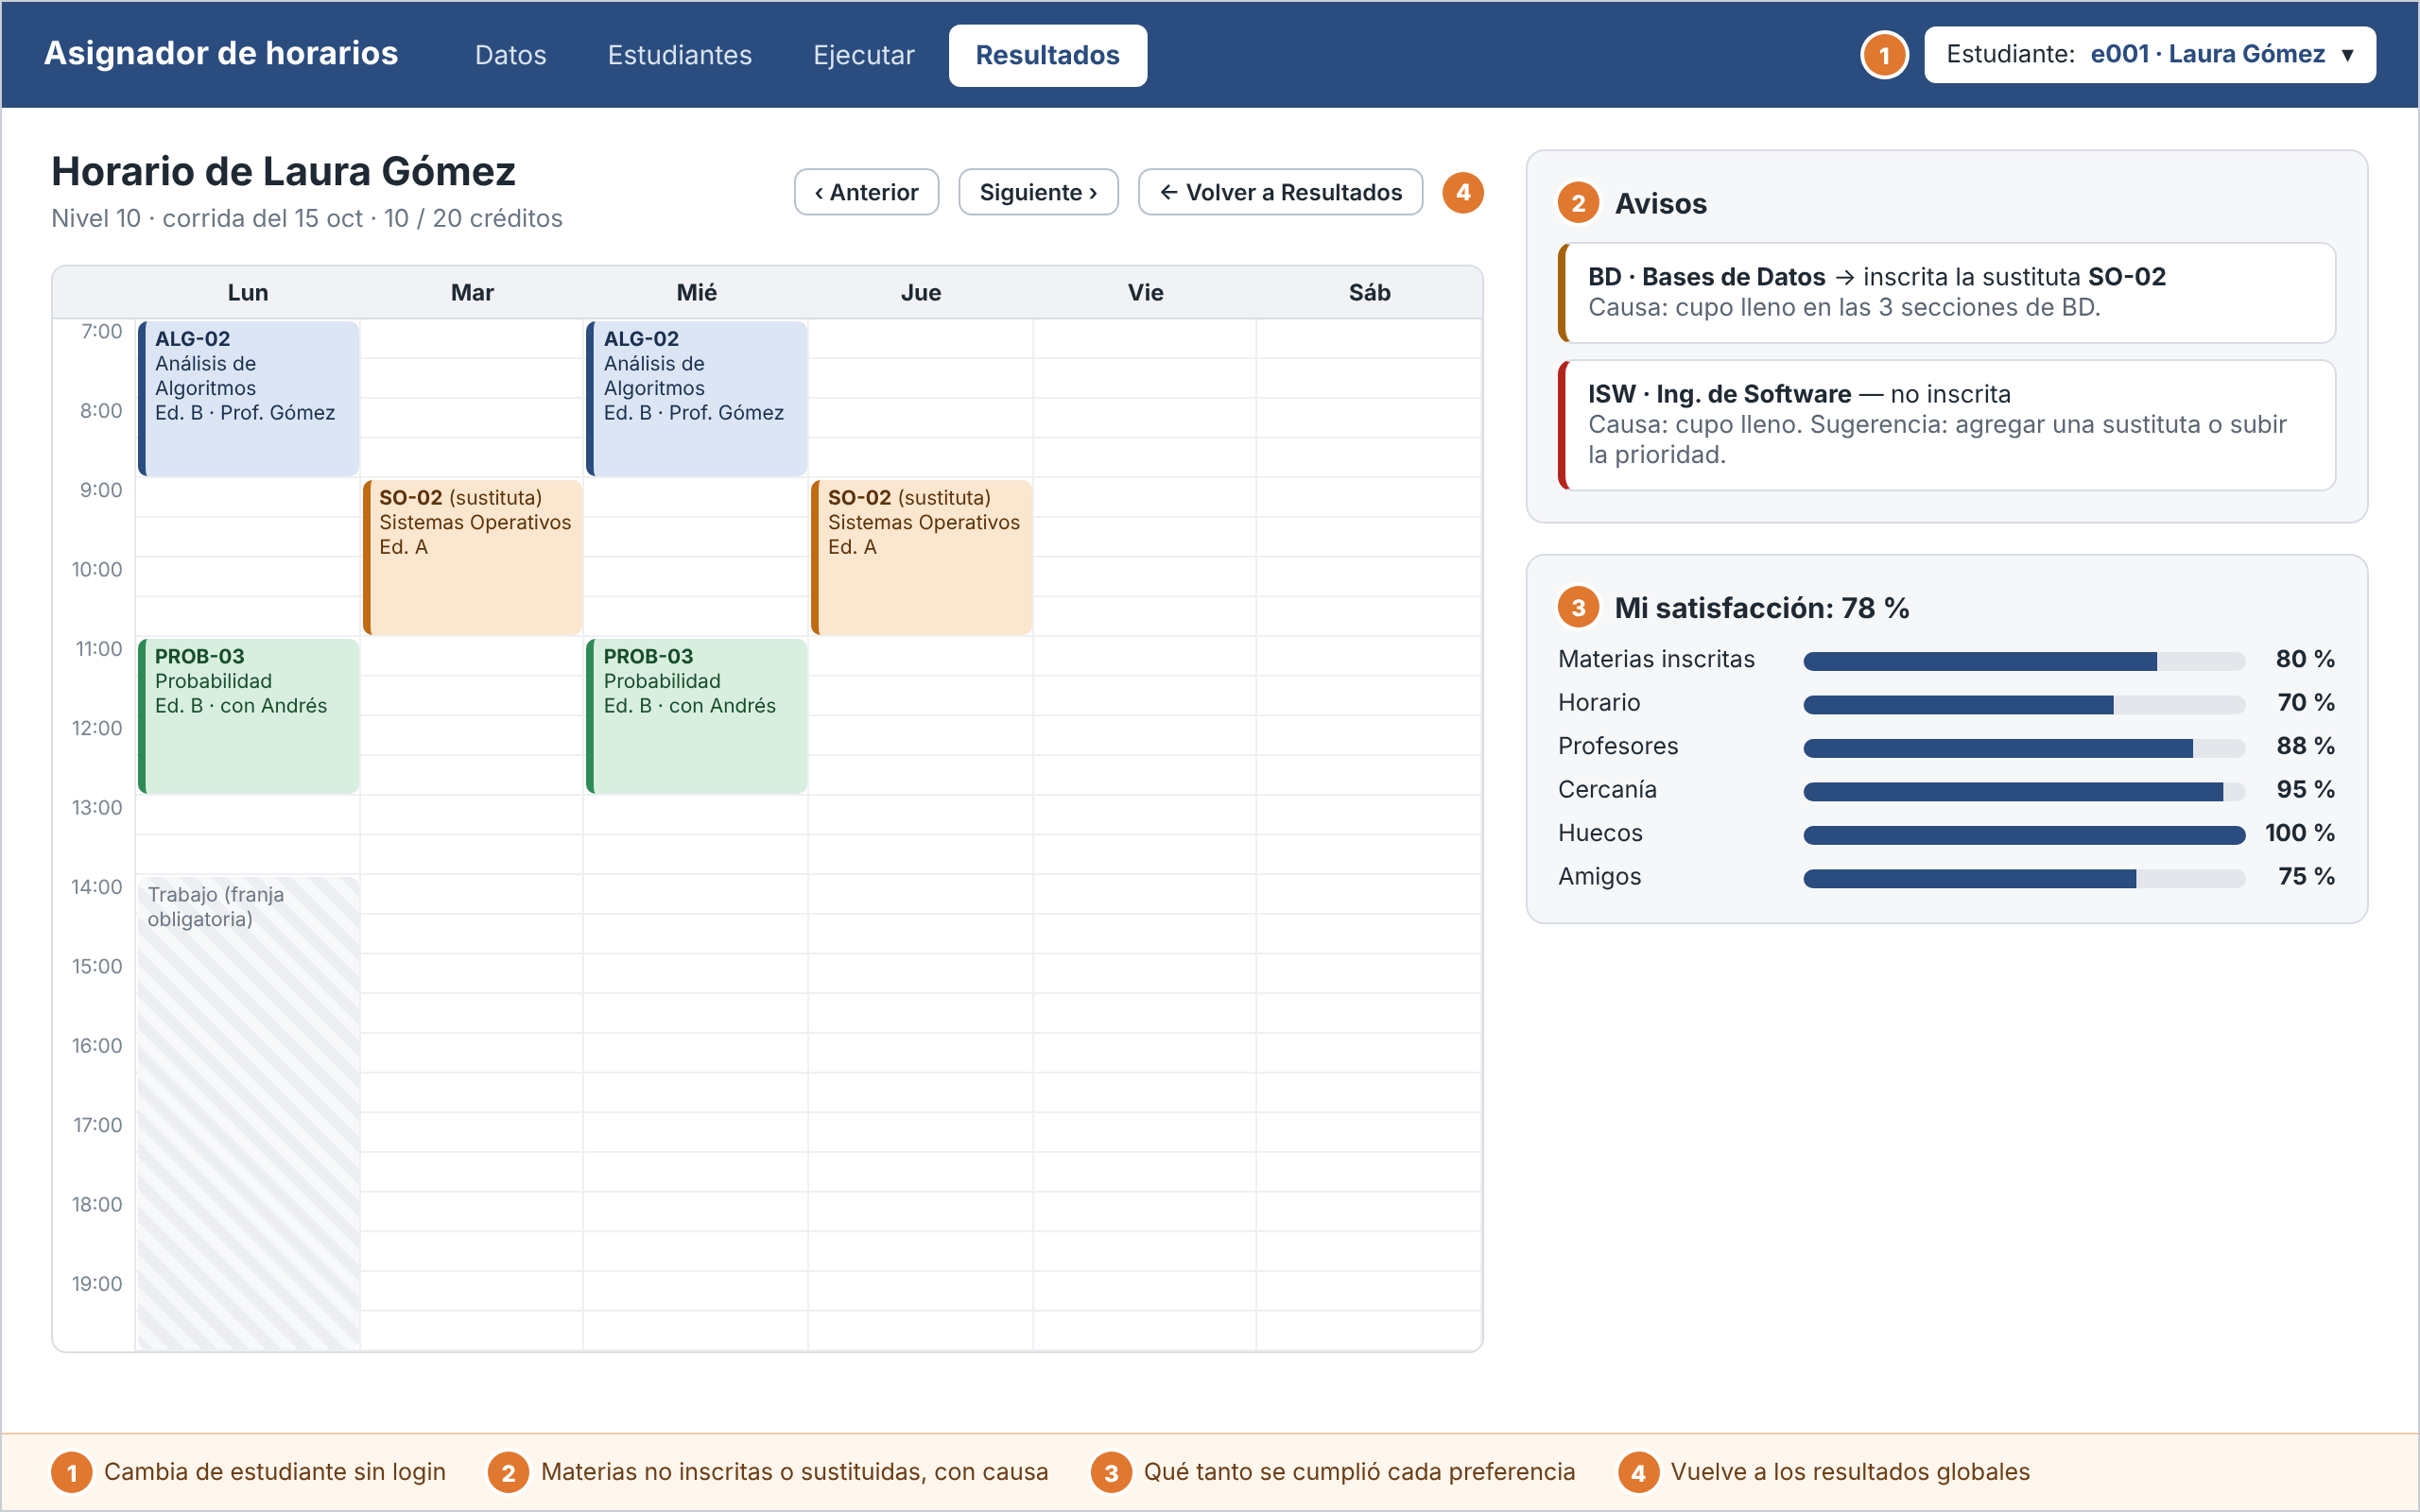
\includegraphics[width=\textwidth]{figuras/mockup6_horario.png}
\caption{Ejemplo de consulta del horario, sustituciones y avisos. Los valores mostrados son ilustrativos.}\label{fig:ui-horario}
\end{figure}

% TODO (Andrés): describir la aplicación implementada (y, si se puede, reemplazar los mockups por capturas reales).
% Indicar si se separaron las etiquetas de materias atendidas y satisfacción, si la carga de datos incluye traslados.json
% y el estado de la pantalla de Preferencias. Borrar la nota en rojo al completar.
\textcolor{red}{[Pendiente: descripción de la aplicación implementada y capturas de pantalla.]}


\FloatBarrier
\bibliography{sn-bibliography}

\end{document}
